\begin{comment}
\documentclass[letterpaper,11pt]{article}
\usepackage{amsfonts,amssymb,amsmath,amsthm,latexsym}
\usepackage[all]{xy}
\usepackage{fullpage}
\usepackage{graphicx}
\usepackage{epstopdf}
\usepackage{epsfig}
\usepackage{hyperref}

\newtheorem{thm}{Theorem}
\newtheorem{lem}{Lemma}
\newtheorem{cor}{Corollary}
\newtheorem{prop}{Proposition}

\theoremstyle{definition}
\newtheorem{defn}{Definition}

\theoremstyle{remark}
\newtheorem{ex}{Example}
\newtheorem{rmk}{Remark}
\newtheorem{exer}{Exercise}

\begin{document}

\newcommand{\CC}{\mathbb{C}}
\newcommand{\RR}{\mathbb{R}}
\newcommand{\ZZ}{\mathbb{Z}}
\newcommand{\PP}{\mathbb{P}}
\newcommand{\fish}{\reflectbox{$\alpha$}}
\newcommand{\Bl}{\text{\rm Bl}}
\newcommand{\PGL}{\text{\rm PGL}}

\title{Cross Ratios}
\date{}
\maketitle

\tableofcontents
\end{comment}

\section{Projective Geometry and Cross ratios}

Projective geometry is the geometry of a painter living in three-dimensional space, who wants to capture what they see on a flat two-dimensional canvas. The symmetries of projective geometry correspond to tilting or rotating the canvas (without the painter moving their head). These symmetries can distort angles and change the ratios between lengths, but at least straight lines will always remain straight.

One important fact about projective geometry is that lines which look parallel on one canvas can meet when projected onto a tilted canvas. Another way of saying this is that two lines in the true three-dimensional world can meet at a point which can't be projected onto the canvas, and the painter's drawings of these lines will appear to be parallel. From the point of view of the canvas, this missing point lives ``at infinity'', but the painter can see the missing point quite clearly. The ``projective plane'' is what we get when we complete the plane of the canvas by adding in the missing points at infinity where parallel lines meet.

\begin{defn} The \emph{projective plane} $\mathbb{P}^2$ is the set of lines through an observation point $O$ in three dimensional space. A \emph{projective line} $l$ is a plane passing through $O$, and a \emph{projective point} $P$ is a line passing through $O$. If the line defining $P$ is contained in the plane defining $l$, we say that $P\in l$.
\end{defn}

The following facts about the projective plane can be verified using standard facts from linear algebra about the dimensions of linear spaces passing through $O$:
\begin{itemize}
\item if $P \ne Q$ are different projective points, then there is exactly one projective line $l$ which contains $P$ and $Q$, and
\item if $l \ne m$ are different projective lines, then there is exactly one projective point $P$ which is contained in both $l$ and $m$.
\end{itemize}
The projective line containing the projective points $P$ and $Q$ is written as $PQ$, and the projective point which is contained in both $l$ and $m$ is written as $l \cap m$. The fact that \emph{every} pair of distinct lines has exactly one intersection point makes the projective plane much easier to work with than the ordinary plane.

If $\mathbb{A}^2$ is an ordinary plane which does not pass through $O$, then we can identify most projective points of $\mathbb{P}^2$ with ordinary points on $\mathbb{A}^2$ by taking the intersection of the line defining the projective point with $\mathbb{A}^2$. The projective line which is defined by a plane passing through $O$ and parallel to $\mathbb{A}^2$ is called the \emph{line at infinity}, or the \emph{horizon line}. Projective points contained in the line at infinity are called \emph{infinite points}.

If we take $O = (0,0,0)$, then we can put coordinates on the projective plane as follows. Every projective point $P$ is a line through $O$ and some other point $(p,q,r)$. Then every point on the line defining $P$ is of the form $(\lambda p,\lambda q,\lambda r)$ for some $\lambda$. We write $P = [p:q:r]$, where the colons indicate that we only care about the ratios of the coordinates. If $\mathbb{A}^2$ is the plane $z=1$, then the ordinary point on $\mathbb{A}^2$ corresponding to $P$ is $(\frac{p}{r},\frac{q}{r},1)$, or if we ignore the $z$-coordinate it is just $(\frac{p}{r},\frac{q}{r})$. If $r = 0$, then $P$ is an infinite point with \emph{slope} $\frac{q}{p}$.

We can define projective coordinates for projective lines as well. A projective line $l$ is defined by a single linear equation
\[
dx+ey+fz = 0,
\]
with not all of $d,e,f$ equal to $0$. Furthermore, this equation defines the same line if all of $d,e,f$ are rescaled by the same nonzero $\lambda$. Thus we say that $l = (d:e:f)$. If $P = [p:q:r]$, then we have $P\in l$ if and only if
\[
dp + eq+ fr = 0.
\]
The intersection of $l$ with the ordinary plane $\mathbb{A}^2$ defined by $z=1$ is just the line $dx+ey+f=0$. The line at infinity has coordinates $(0:0:1)$.

The coordinate system described above can be called \emph{cartesian projective coordinates}. There are other projective coordinate systems, one of the most useful of which is the \emph{barycentric coordinate} system. In the barycentric coordinate system, a triangle $ABC$ in $\mathbb{A}^2$ is fixed and the coordinates of three dimensional space are chosen such that $A=(1,0,0), B = (0,1,0), C = (0,0,1)$ - so the plane $\mathbb{A}^2$ is now defined by the equation $x+y+z = 1$. If $P$ is an ordinary point in $\mathbb{A}^2$, then the projective coordinates $[p:q:r]$ of $P$ are defined to be any three numbers $p,q,r$, not all zero, proportional to the three directed areas $[PBC], [APC], [ABP]$. In the barycentric coordinate system, a line $l=(d:e:f)$ is the set of points $P$ such that
\[
d[PBC] + e[APC] + f[ABP] = 0.
\]
The line at infinity has barycentric coordinates $(1:1:1)$.

\subsection{Cross Ratios}

Before we study the geometry of a painter living in a three-dimensional world with a two-dimensional canvas, we should start by understanding the simpler situation of a painter living in a two-dimensional world who paints on a one-dimensional canvas.

We need to relate the geometry of our one-dimensional canvas to the geometry of what the painter sees, i.e. the geometry of the collection of lines which pass through the painter's eyeball. We'll start with a careful definition of the (signed) ratio, which we will use as a coordinate on a one-dimensional space, analogous to barycentric coordinates.

\begin{defn} If $A,B,C$ are three points on a line, not all equal, then we define their \emph{ratio} to be
\[
(A,B;C) = \frac{AC}{BC},
\]
where the ratio is taken to be positive if the rays $AC$ and $BC$ point in the same direction, and negative otherwise.

If $l_1,l_2,l_3$ are three directed lines passing through a point, not all equal, then their \emph{ratio} is defined by
\[
(l_1,l_2;l_3) = \frac{\sin\angle l_1l_3}{\sin \angle l_2l_3},
\]
where the angles are oriented in the counterclockwise sense.
\end{defn}

\begin{exer}
\begin{itemize}
\item[(a)] Show that if $A\ne B$ then there is a bijection between points $C$ on the line $AB$ and ratios $(A,B;C)$. Thus we can use the ratio as a coordinate on the line $AB$.
\item[(b)] Show that the ratio $(l_1,l_2;l_3)$ does not depend on the orientation of line $l_3$. Show that if $l_1 \ne l_2$ we can use the ratio $(l_1,l_2;l_3)$ as a coordinate on the set of lines through the point $l_1\cap l_2$.
\end{itemize}
\end{exer}

\begin{exer}
Suppose that points $A,B,C$, not all equal, are on a line, and that point $O$ is not on that line. Show that
\[
\frac{(A,B;C)}{(OA,OB;OC)} = \frac{|OA|}{|OB|}.
\]
\end{exer}

\begin{defn} If $A,B,C,D$ are four points on a line, no three of them equal, then we define their \emph{cross ratio} to be
\[
(A,B;C,D) = \frac{(A,B;C)}{(A,B;D)} = \frac{AC}{CB}\bigg/\frac{AD}{DB}.
\]
If $l_1,l_2,l_3,l_4$ are four lines passing through a point, no three of them equal, then their cross ratio is defined by picking an orientation for each line, and then setting
\[
(l_1,l_2;l_3,l_4) = \frac{(l_1,l_2;l_3)}{(l_1,l_2;l_4)} = \frac{\sin\angle l_1l_3}{\sin \angle l_3l_2}\bigg/\frac{\sin\angle l_1l_4}{\sin\angle l_4l_2}.
\]
\end{defn}

\begin{thm}[The fundamental theorem of cross ratios] If $A,B,C,D$ are on a line, no three of them equal, and if $O$ is a point not on that line, then
\[
(OA,OB;OC,OD) = (A,B;C,D).
\]
\end{thm}

We would like to extend the above definitions to any four points or lines in the projective plane. One way to do this is to make special definitions if one of $A,B,C,D$ is an infinite point: for instance, if $\infty$ is the infinite point on line $AB$, then we have
\[
(A,B;C,\infty) = (A,B;C) = -\frac{AC}{CB}.
\]
Similarly, if all of $A,B,C,D$ are infinite points with slopes $a,b,c,d$, then their cross ratio is
\[
(a,b;c,d) = \frac{c-a}{b-c}\bigg/\frac{d-a}{b-d}.
\]
However, the best way to do this is to simply change our canvas to get a coordinate system where none of $A,B,C,D$ is an infinite point. In other words, we find a new plane $\mathbb{A'}^2$ not passing through the observation point $O$, which intersects the four lines corresponding to the projective points $OA,OB,OC,OD$ at some new points $A',B',C',D'$. Then for finite points $A,B,C,D$ we have
\[
(A,B;C,D) = (OA,OB;OC,OD) = (A',B';C',D'),
\]
so the cross ratio in the new coordinate system will be the same as the original cross ratio. If one of $A,B,C,D$ is an infinite point we use this formula as the \emph{definition} of the cross ratio.

To check your understanding, calculate the cross ratio of four parallel lines in terms of the distances between them (parallel lines intersect at the infinite point corresponding to their common slope).

\begin{exer} Let $ABC$ be a triangle, let $M$ be the midpoint of $AC$, and let $N$ be a point on line $BM$ such that $AN$ is parallel to $BC$. Let $P$ be any point on line $AC$, and let $Q$ be the intersection of line $BP$ with line $AN$. Use cross ratios to prove that
\[
\frac{AQ}{QN} = \frac{1}{2}\frac{AP}{PM}.
\]
\end{exer}

\begin{exer} Suppose a painter is painting a square-tiled floor which he is looking at from an angle. Given that the painter draws the four corners of one of the squares at the four points $ABCD$, construct the rest of the points that the painter draws using only a straightedge. If the next two points that the painter draws along the line $AB$ are $X$ and $Y$, compute the value of the cross ratio $(A,B;X,Y)$.
\end{exer}

\begin{exer}
\begin{itemize}
\item[(a)] Check that for any number $\lambda$ we have $(\lambda,1;0,\infty) = \lambda$.
\item[(b)] Show that $(A,B;D,C) = \frac{1}{(A,B;C,D)}$.
\item[(c)] Show that $(A,C;D,B) = \frac{1}{1-(A,B;C,D)}$.
\end{itemize}
\end{exer}

\begin{exer}
\begin{itemize}
\item[(a)] Show that if $A\ne B$ and $(A,B;C,X) = (A,B;C,Y)$ then $X=Y$.
\item[(b)] Show that if $(A,B;C,D) = 1$ then either $A=B$ or $C=D$.
\item[(c)] Show that if $A\ne B$, $C\ne D$, and $(A,B;C,D) = (A,B;D,C)$ then $(A,B;C,D) = -1$.
\end{itemize}
\end{exer}

\begin{defn} If $(A,B;C,D) = -1$, then the four points $A,B,C,D$ are called \emph{harmonic}. We also say that $D$ is the \emph{harmonic conjugate} of $C$ with respect to $A,B$. Sometimes we say that $A,B,C,D$ are harmonic when three of them are equal.
\end{defn}

\begin{ex}
\begin{itemize}
\item[(i)] If $M$ is the midpoint of $AB$ and if $\infty$ is the infinite point along line $AB$, then $(A,B;M,\infty) = -1$.

\item[(ii)] If $ABC$ is a triangle, and if $X,Y$ are the feet of the internal and external angle bisectors through $C$, then $(A,B;X,Y) = -1$ by the angle bisector theorem.

\item[(iii)] We have $(1,-1;x,\frac{1}{x}) = -1$ and $(0,\infty;x,-x) = -1$ for any $x$.
\end{itemize}
\end{ex}

\begin{figure}[!htb]
\centering
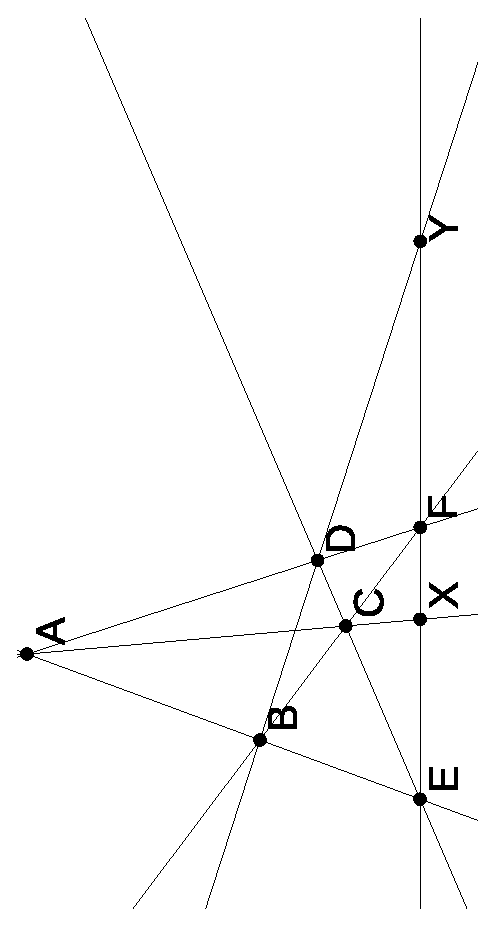
\includegraphics[scale=0.7,angle=270]{quad.eps}
\caption{Quadrilateral Theorem}
\end{figure}

\begin{thm}[Quadrilateral Theorem] Let $ABCD$ be any quadrilateral. Let $E$ be the intersection of sides $AB$ and $CD$, and let $F$ be the intersection of sides $BC$ and $DA$. Let $X$ be the intersection of diagonal $AC$ with the line $EF$, and let $Y$ be the intersection of diagonal $BD$ with line $EF$. Then
\[
(E,F;X,Y) = -1.
\]
\end{thm}
\begin{proof}[Proof 1, using Ceva and Menelaus] By Ceva applied to triangle $AEF$ and point $C$, we have
\[
\frac{AB}{BE}\frac{EX}{XF}\frac{FD}{DA} = 1.
\]
By Menelaus applied to triangle $AEF$ and line $BD$, we have
\[
\frac{AB}{BE}\frac{EY}{YF}\frac{FD}{DA} = -1.
\]
Dividing these two equations, we get $(E,F;X,Y) = -1$.
\end{proof}
\begin{proof}[Proof 2, using cross ratios] Let $P$ be the intersection of the diagonals $AC$ and $BD$. We have
\[
(E,F;X,Y) = (AE,AF;AX,AY) = (B,D;P,Y) = (CB,CD;CP,CY) = (F,E;X,Y).
\]
Since $E\ne F$ and $X\ne Y$, we conclude that $(E,F;X,Y) = -1$.
\end{proof}

If $EA,EB,EC,ED$ intersect a line $l$ at points $A',B',C',D'$, it often saves space to abbreviate the inference
\[
(A,B;C,D) = (EA,EB;EC,ED) = (A',B';C',D')
\]
by just writing
\[
(A,B;C,D) \stackrel{E}{=} (A',B';C',D').
\]
Now let's use this notation to give a compact proof of Desargues' Theorem:

\begin{thm}[Desargues' Theorem]\label{desargues} Suppose that triangles $ABC$ and $XYZ$ are \emph{perspective from a point}, that is, suppose that the lines $AX,BY,CZ$ all meet at a point $P$. Then the triangles $ABC$ and $XYZ$ are \emph{perspective from a line}, that is, the intersections $AB\cap XY$, $BC\cap YZ$, $CA\cap ZX$ all lie on a line.
\end{thm}
\begin{proof}
Let $U = BC\cap YZ$, $V = CA\cap ZX$, $W = AB\cap XY$. We want to show that $U,V,W$ lie on a line, so we may as well suppose that $V\ne W$. Let $Q,M,N$ be the intersections of line $BY$ with the lines $WV$, $AC$, $XZ$, respectively. Then we have
\[
(W,V;Q,BC\cap VW) \stackrel{B}{=} (A,V;M,C) \stackrel{P}{=} (X,V;N,Z) \stackrel{Y}{=} (W,V;Q,YZ\cap VW).
\]
Thus $BC\cap VW = YZ\cap VW$, so the three lines $BC,YZ,VW$ meet at the point $U$.
\end{proof}

\begin{figure}[!htb]
\centering
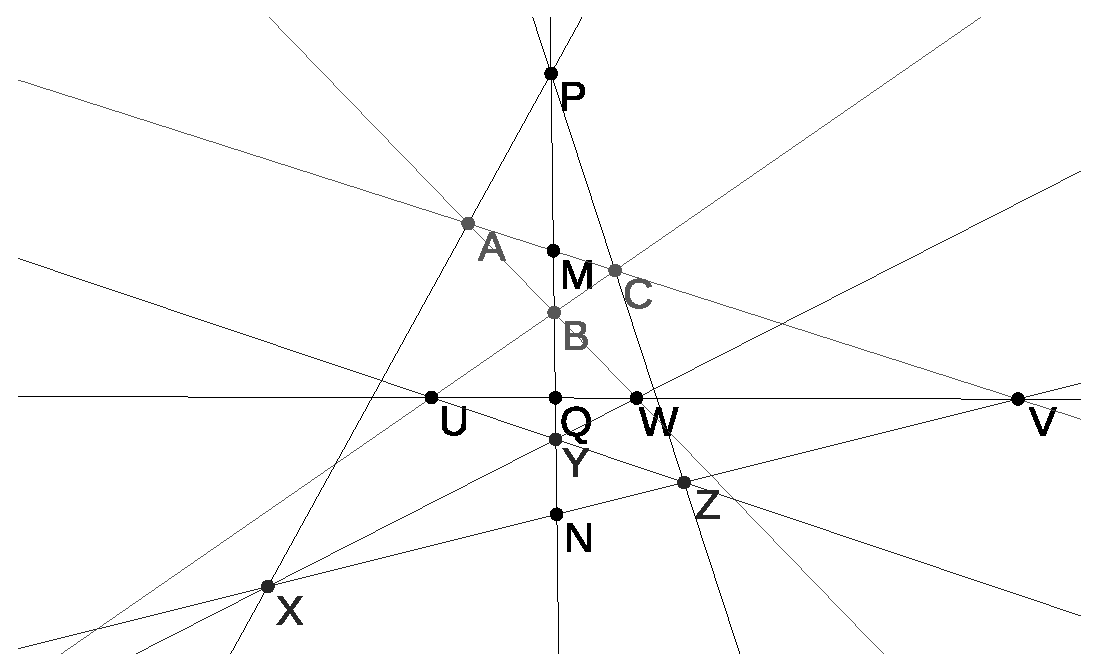
\includegraphics[scale=0.7]{desargues.eps}
\caption{Desargues' Theorem}
\end{figure}

\begin{exer}[Pappus's Hexagon Theorem] Let $A,B,C$ be on a line, and let $D,E,F$ be on another line. Let $X = AE\cap BD, Y = BF\cap CE, Z = CD\cap AF$. Use cross ratios to show that $X,Y,Z$ are on a line. (Hint: let $P = CD\cap BF$, and show that $(C,D;P,Z) = (C,D;P,CD\cap XY)$.)
\end{exer}

\begin{thm}[Cross Ratio Equality]\label{cr-equal} Let $A,B,C,D$ be on a line, and let $E,F,G,H$ be on another line. Let $X = AF\cap BE, Y = BG\cap CF, Z = CH\cap DG$. Then $X,Y,Z$ are on a line if and only if $(A,B;C,D) = (E,F;G,H)$.
\end{thm}
\begin{figure}[!htb]
\centering
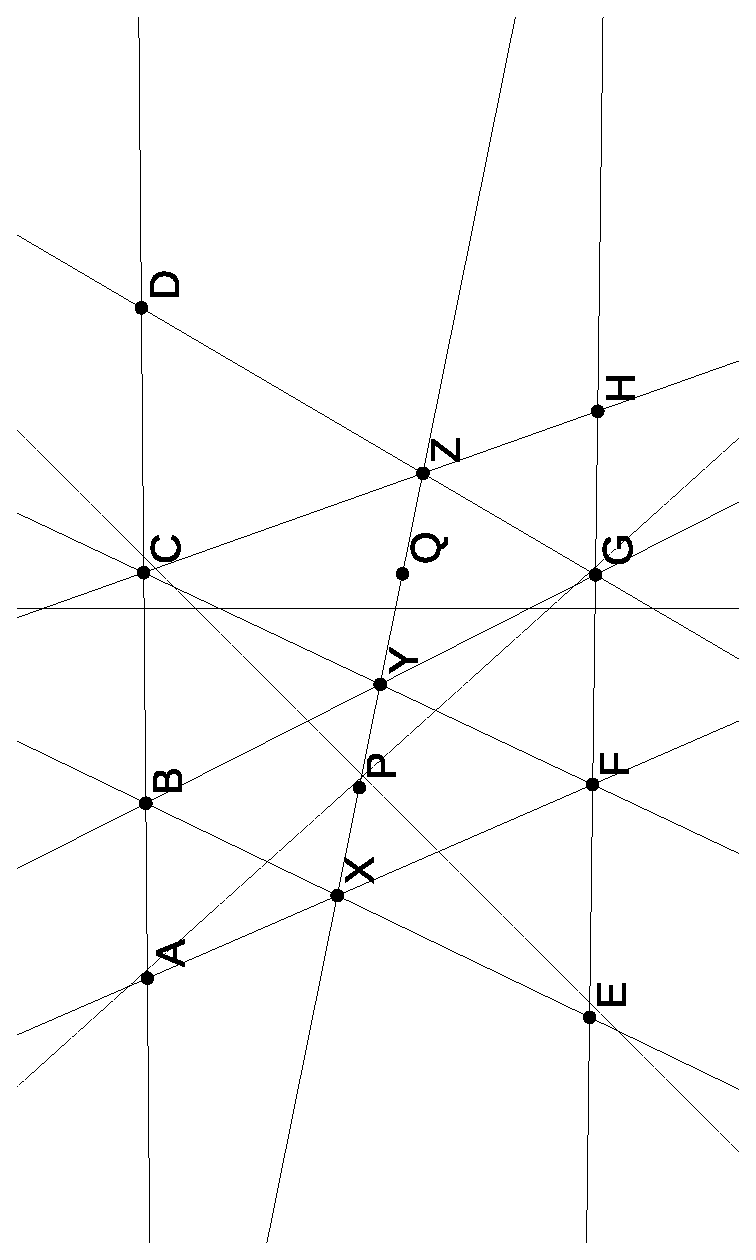
\includegraphics[scale=.5,angle=270]{equal.eps}
\caption{Equal cross ratios}
\end{figure}
\begin{proof} Let $P = AG\cap CE, Q = CG\cap XY$. By Pappus's Theorem, $P$ is on line $XY$. Projecting through $G$, we have $(A,B;C,D) \stackrel{G}{=} (P,Y;Q,DG\cap XY)$, and projecting through $C$, we have $(E,F;G,H) \stackrel{C}{=} (P,Y;Q,CH\cap XY)$. Thus $(A,B;C,D) = (E,F;G,H)$ if and only if $CH, DG$, and $XY$ meet at a point.
\end{proof}

\subsection{Cross Ratios on a Conic Section}

\begin{prop} Suppose that $A,C,B,D$ are on circle $\omega$, and that the (directed) arcs $AC,CB,BD,DA$ of $\omega$ have central angles $2\alpha,2\beta,2\gamma,2\delta$. Let $E$ be any other point on $\omega$. Then
\[
(EA,EB;EC,ED) = -\frac{\sin \alpha}{\sin \beta}\bigg/\frac{\sin \delta}{\sin \gamma}.
\]
In particular, we have
\[
(EA,EB;EC,ED) = \pm\frac{|AC||BD|}{|AD||BC|},
\]
where the sign is negative if and only if the points $A,B$ separate the points $C,D$.
\end{prop}

\begin{cor} Let $\omega$ be any \emph{conic section}, that is, any intersection of a cone $\mathcal{C}$ through the observation point $O$ with the plane $\mathbb{A}^2$. If $A,B,C,D,E,F$ are any six points on $\omega$, then we have
\[
(EA,EB;EC,ED) = (FA,FB;FC,FD).
\]
\end{cor}
\begin{proof} First we prove it when $\omega$ is a circle. By Proposition 2, we have
\[
(EA,EB;EC,ED) = -\frac{\sin \alpha}{\sin \beta}\bigg/\frac{\sin \delta}{\sin \gamma} = (FA,FB;FC,FD).
\]
For the general case, we choose another plane $\mathbb{A'}^2$ such that $\mathcal{C}\cap\mathbb{A'}^2$ is a circle. Let $A',B',...$ be the intersections of lines $OA,OB, ...$ with the plane $\mathbb{A'}^2$. Then we have
\[
(EA,EB;EC,ED) \stackrel{O}{=} (E'A',E'B';E'C',E'D') = (F'A',F'B';F'C',F'D') \stackrel{O}{=} (FA,FB;FC,FD).\qedhere
\]
\end{proof}

\begin{defn} If $A,B,C,D$ are four points on a conic section $\omega$, then we define the cross ratio of $A,B,C,D$ with respect to $\omega$ by choosing any fifth point $E$ on $\omega$ and setting
\[
(A,B;C,D)_{\omega} = (EA,EB;EC,ED).
\]
By Corollary 2, this doesn't depend on the choice of $E$.
\end{defn}

\begin{exer} Check that the cross-ratio formula $(A,B;C,D)_\omega = 1 - (A,C;B,D)_\omega$ is equivalent to Ptolemy's theorem when $\omega$ is a circle.
\end{exer}

\begin{rem} The concept of \emph{separation} can be defined on lines and conics as follows: we say that the points $A,B$ separate the points $C,D$ on $\omega$ if deleting the points $A,B$ from $\omega$ cuts $\omega$ into two disconnected components, one of which contains $C$ and the other of which contains $D$. To make sense of this definition on a hyperbola, parabola, or line, it is necessary to include the points at infinity in the conic $\omega$. Then we have
\[
(A,B;C,D)_\omega < 0
\]
exactly when the points $A,B$ separate the points $C,D$ on $\omega$.

Separation is the fundamental ordering-like concept which is appropriate when we study real projective geometry. For Euclidean geometry, the analogous concept is \emph{betweenness}: if $A,B,C$ lie on a line $\ell$, then we say that $C$ is between $A$ and $B$ when deleting $C$ from $\ell$ cuts $\ell$ into two disconnected components (ignoring the point at infinity), one of which contains $A$ and the other of which contains $B$. Betweenness is a special case of separation: $C$ is between $A,B$ on the line $\ell$ exactly when the points $A,B$ separate the points $C,\infty_\ell$ along $\ell$. There turn out to be exactly four fundamental ordering-like concepts on lines and circles:
\begin{itemize}
\item order, for two points on a directed line,
\item betweenness, for three points on an undirected line,
\item cyclic order, for three points on an oriented circle, and
\item separation, for four points on an unoriented circle.
\end{itemize}
Each of these concepts has an elegant axiomatic system which goes along with it. Facts about betweenness are often used without explicit mention in Euclidean geometry, and were left out of Euclid's five axioms for geometry but included in Hilbert's more careful list of axioms for geometry. In two-dimensional Euclidean geometry, the main nontrivial fact about betweenness is called \emph{Pasch's axiom}, which states that if a line meets one side of a triangle internally, then it meets one of the other two sides of the triangle internally.
\end{rem}

Our first application of the cross ratio on a conic is to give a short proof of Pascal's theorem.

\begin{figure}[!htb]
\centering
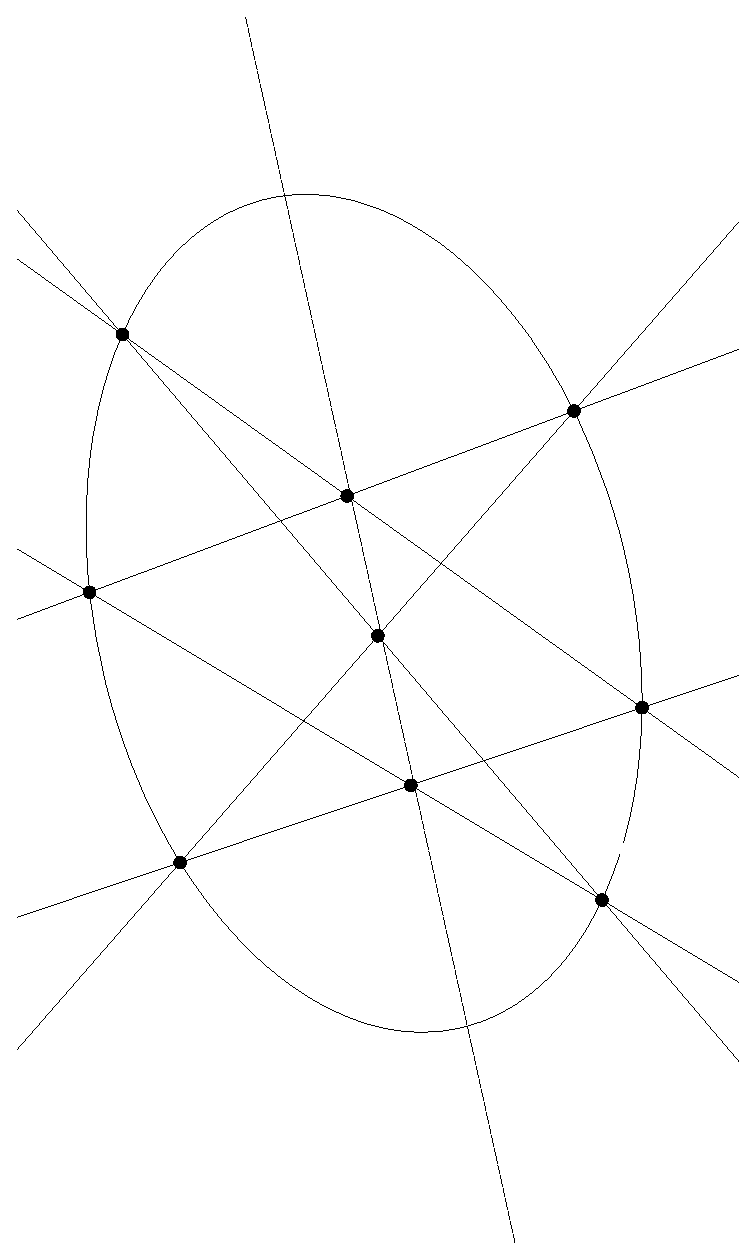
\includegraphics[scale=.5,angle=90]{pascal.eps}
\caption{Pascal's Theorem}
\end{figure}

\begin{thm}[Pascal's Theorem] If $ABCDEF$ is any hexagon with vertices lying on a conic $\omega$, then the three intersections of opposite sides $AB\cap DE$, $BC\cap EF$, $CD\cap FA$ lie on a line.
\end{thm}
\begin{proof} Let $L = BC\cap EF$, $M = CD\cap FA$, $N = AB\cap DE$ be the intersections of opposite sides of the hexagon. Let $P = AF\cap BC$ and $Q = AB\cap CD$. Then
\[
(C,L;P,B) \stackrel{F}{=} (C,E;A,B)_{\omega} \stackrel{D}{=} (Q,N;A,B) \stackrel{M}{=} (C,MN\cap BC;P,B).
\]
Thus $L = MN\cap BC$, so $L$ is on the line $MN$.
\end{proof}

\begin{exer}\label{conicline}\hspace{2em}
\begin{itemize}
\item[(a)] Given points $A,B,C,D,E$ and a line $l$ through $A$ construct, using only a straightedge, the second point of intersection $F$ between the line $l$ and the conic through the points $A,B,C,D,E$.

\item[(b)] Given points $A,B,C,D,E$ construct, using only a straightedge, the line $l$ which is tangent to the conic through the points $A,B,C,D,E$ at $A$.
\end{itemize}
\end{exer}

\begin{exer} Suppose points $A,B,C,D,E,F,G,H$ lie on a conic $\omega$. Let $X = AF\cap BE, Y = BG\cap CF, Z = CH\cap DG$. Show that $(A,B;C,D)_\omega = (E,F;G,H)_\omega$ if and only if $X,Y,Z$ are on a line.
\end{exer}

Another easy application is a short proof of the butterfly theorem.

\begin{figure}[!htb]
\centering
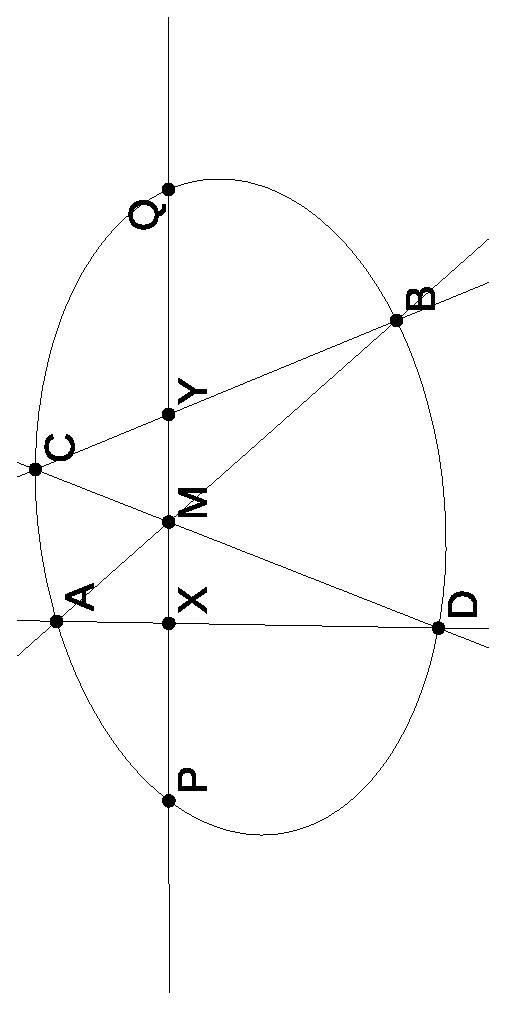
\includegraphics[scale=.5,angle=270]{butterfly.eps}
\caption{The Projective Butterfly Theorem}
\end{figure}

\begin{thm}[Projective Butterfly Theorem]\label{butterfly} Let $\omega$ be a conic, and let $PQ$ be a chord on $\omega$ through the point $M$. Let $AB$ and $CD$ be two more chords of $\omega$ passing through $M$, and set $X = AD\cap PQ, Y = BC\cap PQ$. Then $(P,Q;M,X) = (Q,P;M,Y)$. In particular, if $M$ is the midpoint of $PQ$ then $|MX| = |MY|$.
\end{thm}
\begin{proof}
\[
(P,Q;M,X) \stackrel{A}{=} (P,Q;B,D)_{\omega} \stackrel{C}{=} (P,Q;Y,M) = (Q,P;M,Y).
\]
We leave the proof of the last claim as an easy exercise to the reader.
\end{proof}

\begin{defn} A cyclic quadrilateral $ACBD$ is called \emph{harmonic} if $A\ne B, C\ne D$, and $|AC||BD| = |AD||BC|$.
\end{defn}

\begin{exer}\label{harmquad}
\begin{itemize}
\item[(a)] Suppose $P$ is a point outside circle $\omega$. Let the two tangents from $P$ to $\omega$ meet $\omega$ at $A$ and $B$. Let $l$ be a line through $P$ meeting $\omega$ at two points $C$ and $D$. Show that $ACBD$ is a harmonic quadrilateral.

\item[(b)] Let $P,\omega,A,B,C,D$ be as in (a), and let $Q$ be the intersection of $AB$ and $CD$. Show that $(C,D;P,Q) = -1$.

\item[(c)] Let $P,\omega,A,B$ be as in (a). Show that $P'$, the inverse $P$ with respect to $\omega$, is on the line $AB$.
\end{itemize}
\end{exer}

\begin{exer} Let $\omega$ be the unit circle, given in affine coordinates by the equation $x^2+y^2 = 1$. Let $A = (1,0), B = (0,1), C = (-1,0)$ in affine coordinates. Find the affine coordinates of the point $D$ on $\omega$ such that $ACBD$ is a harmonic quadrilateral.
\end{exer}

\begin{exer} Let $ABCDE$ be a regular pentagon inscribed in a circle $\omega$. Compute $(A,B;C,D)_\omega$.
\end{exer}

\begin{figure}[!htb]
\centering
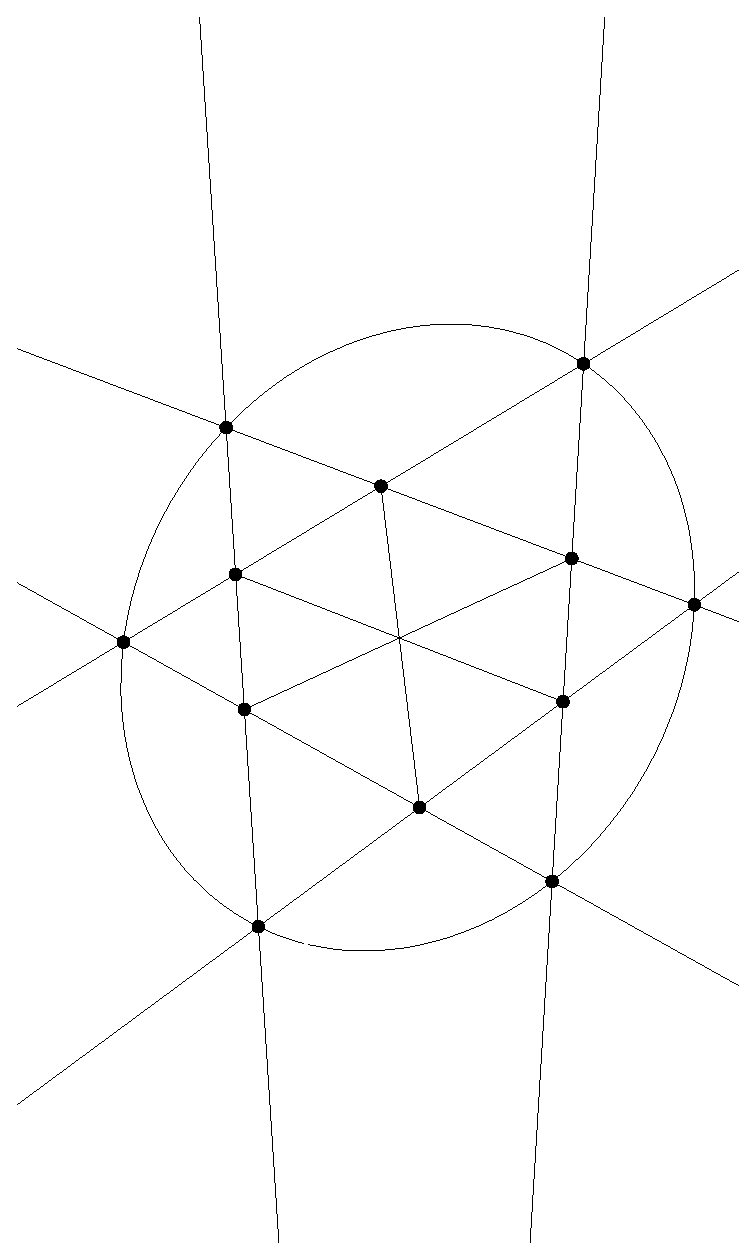
\includegraphics[scale=0.5,angle=270]{conicexer.eps}
\caption{Exercise \ref{conic-exer}}
\end{figure}

\begin{exer}\label{conic-exer} Let $A,B,C,D,E,F$ be six distinct points in the plane. Let $U = BC\cap DE, V = CA\cap EF, W = AB\cap FD, X = AB\cap EF, Y = BC\cap FD, Z = CA\cap DE$, so that hexagon $UZVXWY$ is the intersection of triangles $ABC$ and $DEF$ if it is convex. Show that the lines $UX,VY,WZ$ meet in a point if and only if the points $A,B,C,D,E,F$ lie on a conic.
\end{exer}

\subsection{Cross Ratios on the Inversive Plane}

Just as we used three projective coordinates for the projective plane, we use two projective coordinates to describe a projective line. Specifically, the projective point $[s:t]$ will correspond to the ordinary point with coordinate $z = \frac{s}{t}$ if $t\ne 0$, and to the point $\infty$ if $t=0$. When we allow $s,t$ to be \emph{complex} numbers, we get what is sometimes called the \emph{complex projective line} $\mathbb{CP}^1$, the \emph{inversive plane}, or the \emph{Riemann sphere}.

We define cross ratios on the inversive plane the same way we define cross ratios on a line:
\[
(a,b;c,d) = \frac{c-a}{b-c}\bigg/\frac{d-a}{b-d},
\]
where now $a,b,c,d$ are complex numbers corresponding to ordinary points $A,B,C,D$ in the inversive plane.

\begin{prop} The points $A,B,C,D$ corresponding to the complex numbers $a,b,c,d$ are on a circle or a line if and only if $(a,b;c,d)$ is a real number. If they are on a line, we have $(a,b;c,d) = (A,B;C,D)$, and if they are on a circle $\omega$, we have $(a,b;c,d) = (A,B;C,D)_{\omega}$.
\end{prop}
\begin{proof} Left as an exercise.
\end{proof}

Inversion around the unit circle is given by the simple formula $z\mapsto \frac{1}{\bar{z}}$ in the inversive plane. We have
\[
\left(\frac{1}{\bar{a}},\frac{1}{\bar{b}};\frac{1}{\bar{c}},\frac{1}{\bar{d}}\right) = \overline{\frac{\frac{1}{c}-\frac{1}{a}}{\frac{1}{b}-\frac{1}{c}}\bigg/\frac{\frac{1}{d}-\frac{1}{a}}{\frac{1}{b}-\frac{1}{d}}} = \overline{\frac{a-c}{c-b}\bigg/\frac{a-d}{d-b}} = \overline{(a,b;c,d)},
\]
so inversion takes cross ratios to their complex conjugates. As a consequence, we see that inversion takes circles and lines to circles and lines, and furthermore it takes harmonic quadrilaterals to harmonic quadrilaterals.

\begin{defn} To every two by two matrix $M=\left(\begin{array}{cc}a & b\\ c & d\end{array}\right)$ with determinant $ad-bc$ not equal to zero, we associate a transformation $f_M$ of the inversive plane as follows. In projective coordinates $[s:t]$, we write
\[
f_M([s:t]) = [as+bt:cs+dt].
\]
In ordinary coordinates $z = \frac{s}{t}$, we write
\[
f_M(z) = \frac{az+b}{cz+d}.
\]
The maps $f_M$ are called \emph{M\"obius Transformations}.
\end{defn}

\begin{exer} Show that for any two by two matrix $M$ with nonzero determinant, and for any four points $a,b,c,d$ on the inversive plane, we have
\[
(f_M(a),f_M(b);f_M(c),f_M(d)) = (a,b;c,d).
\]
\end{exer}

\begin{exer} Check that composition of M\"obius transformations corresponds to matrix multiplication, i.e. that for any two matrices $M,N$ and any point $[s:t]$ we have
\[
f_M(f_N([s:t])) = f_{MN}([s:t]).
\]
\end{exer}

\begin{exer} Let $A,B,C,X,Y,Z$ be six points on the projective line, no two of $A,B,C$ equal and no two of $X,Y,Z$ equal. Prove that there is a M\"obius transformation $f$ such that $f(A) = X, f(B) = Y, f(C) = Z$.
\end{exer}

\subsection{Invertible functions on the line}

Suppose a projective line $\mathbb{P}^1$ has coordinate $z$, and we have defined an invertible map $f:\mathbb{P}^1 \rightarrow \mathbb{P}^1$ via some geometric procedure that has no ``configuration issues'' (so for instance, taking the \emph{leftmost} intersection of a circle with a line would not count). Since any geometrically defined map can be described algebraically by writing every point out in coordinates, our function $f$ may be written as an algebraic function of $z$, and if there are no ``configuration issues'', then $f$ must be a rational function, i.e. a ratio of two polynomials:
\[
f(z) = \frac{p(z)}{q(z)}.
\]
Since $f$ is invertible, the equation $f(z) = w$ should have exactly one solution, so the polynomial
\[
p(z) - wq(z)
\]
should have degree $1$ for every constant $w$. Thus $p$ and $q$ are both linear polynomials, and we can write
\[
f(z) = \frac{az+b}{cz+d}.
\]
Thus, $f$ is in fact a M\"obius transformation, and so $f$ preserves the cross ratio. We record this as an informal theorem.

\begin{thm}\label{invariant} If $f$ is an invertible function from a line to a line that is defined by a geometric procedure that has no ``configuration issues'', then $f$ preserves the cross ratio. Furthermore, in this case $f$ is a M\"obius transformation.
\end{thm}

\begin{exer} Prove the converse: if $f:\mathbb{P}^1 \rightarrow \mathbb{P}^1$ is any function that preserves the cross ratio, prove that $f$ is a M\"obius transformation, and find a geometric construction of the function $f$.
\end{exer}

As an application, we consider the harmonic conjugation map. For any points $A,B$ on $\mathbb{P}^1$, we define
\[
h_{A,B}(C) = D\mbox{ if }(A,B;C,D) = -1.
\]
We can construct $D$ geometrically using the Quadrilateral Theorem, and $h_{A,B}$ is clearly invertible, so by the above discussion $h_{A,B}$ is a M\"obius transformation. In coordinates, if $A$ has coordinate $a$ and $B$ has coordinate $b$, we have
\[
h_{a,b}(z) = \frac{(a+b)z-2ab}{2z-a-b}.
\]
Harmonic conjugation has the property that $h_{A,B}(h_{A,B}(C)) = C$ - in other words, harmonic conjugation is always an \emph{involution}. In fact, this property characterizes harmonic conjugation.

\begin{thm} If $f$ is a M\"obius transformation with the further property that $f$ is an involution, i.e. $f(f(C)) = C$ for all points $C$, then $f$ is either the identity map or there is a pair of (possibly imaginary) points $A,B$ such that $f = h_{A,B}$.
\end{thm}
\begin{proof} In coordinates, the equation $f(z) = z$ becomes a quadratic after clearing the denominator. If $f$ is not the identity map, this quadratic will have two solutions, corresponding to two distinct points $A,B$. For any point $C$, write $D = f(C)$. Since $f$ preserves the cross ratio, we have
\[
(A,B;C,D) = (f(A),f(B);f(C),f(D)) = (A,B;D,C),
\]
so the points $A,B,C,D$ are harmonic.
\end{proof}

\subsection{Angles and the circle points}

Two special points in the projective plane allow us to talk about angles using cross ratios. These points are both infinite and imaginary, but we can treat them the same way we treat any other points in projective geometry. This allows us to solve many problems that are traditionally thought to be out of the scope of projective geometry.

\begin{defn} The \emph{circle points} are the points $\fish = [i:1:0]$ and $\bar\fish = [1:i:0]$. These are the points at infinity of slope $-i$ and $i$.
\end{defn}

I used the symbols $\fish$ and $\bar\fish$ for the circle points, since some people might find points which are both infinite and imaginary to be slightly fishy.

\begin{thm}[Angle Theorem] If lines $l, m$ intersect the line at infinity in points $L,M$, then
\[
(L,M;\fish,\bar\fish) = e^{2i\angle lm}.
\]
In particular, lines $l$ and $m$ are orthogonal if and only if points $L,M,\fish,\bar\fish$ are harmonic.
\end{thm}
\begin{proof} Let $s$ be the slope of line $l$ and let $t$ be the slope of line $m$. By the tangent subtraction formula, we have
\[
\tan(\angle lm) = \frac{t-s}{1+st}.
\]
We have
\begin{align*}
(L,M;\fish,\bar\fish) &= (s,t;-i,i)\\
&= \frac{s+i}{-i-t}\bigg/\frac{s-i}{i-t}\\
&= \frac{(s+i)^2(t-i)^2}{(s^2+1)(t^2+1)}\\
&= \frac{(st+1)^2 - (t-s)^2 + 2i(t-s)(st+1)}{(st+1)^2 + (t-s)^2}\\
&= \frac{1-\tan^2(\angle lm)}{1+\tan^2(\angle lm)} + i\frac{2\tan(\angle lm)}{1+\tan^2(\angle lm)}\\
&= \cos(2\angle lm) + i\sin(2\angle lm)\\
&= e^{2i\angle lm}.\qedhere
\end{align*}
\end{proof}

\begin{thm} A conic $\omega$ is a circle if and only if it passes through the two circle points.
\end{thm}
\begin{proof} First, suppose $\omega$ is a circle with center $(a,b)$ and radius $r$. In projective coordinates, $\omega$ is the set of points $[x:y:z]$ such that
\[
(x-az)^2 + (y-bz)^2 = (rz)^2.
\]
Plugging in, we can check that $[x:y:z] = [i:1:0]$ and $[x:y:z] = [1:i:0]$ satisfy the equation defining $\omega$.

Now suppose $\omega$ is any conic passing through $\fish,\bar\fish$. Let $A,B,C,D$ be any four points on $\omega$. Then we have
\[
e^{2i\angle CAD} = (AC,AD;A\fish,A\bar\fish) = (C,D;\fish,\bar\fish)_{\omega} = (BC,BD;B\fish,B\bar\fish) = e^{2i\angle CBD},
\]
so the directed angles $\angle CAD$ and $\angle CBD$ are congruent modulo $\pi$. Thus $A,B,C,D$ are concyclic.
\end{proof}

\begin{cor} Let $A,B$ be two points on a circle $\omega$ with center $O$. Then
\[
(A,B;\fish,\bar\fish)_\omega = e^{i\angle AOB}.
\]
In particular, if $A,B$ are diametrically opposite then $A,B,\fish,\bar\fish$ are harmonic.
\end{cor}

\begin{exer}\label{melodic} Say that four distinct points $A,B,C,D$ on a line are \emph{melodic} if we have
\[
(A,B;C,D) = (A,D;B,C),
\]
and make a similar definition for four points on a conic. Let $ABCDEF$ be a regular hexagon inscribed in a circle $\omega$. Prove that the four points $A,B,\fish,\bar\fish$ are melodic with respect to $\omega$.
\end{exer}

% TODO: First isodynamic point is melodic

\subsection{Polar maps}

\begin{defn} We say that two points $P,Q$ are \emph{harmonic conjugates} with respect to a conic $\omega$ if $P,Q,X,Y$ are harmonic, where $X,Y$ are the (possibly imaginary) points of intersection of $\omega$ and $PQ$.
\end{defn}

\begin{thm} Let $P$ be a point and $\omega$ a conic. Then the locus $p$ of harmonic conjugates of $P$ with respect to $\omega$ is a line.
\end{thm}
\begin{proof}[Proof 1, using tangents] Let $U,V$ be the feet of the two tangents from $P$ to $\omega$. We will show that every point $Q$ on the line $UV$ is a harmonic conjugate of $P$ with respect to $\omega$. Let the line $PQ$ meet $\omega$ at $X,Y$.

\begin{figure}[!htb]
\centering
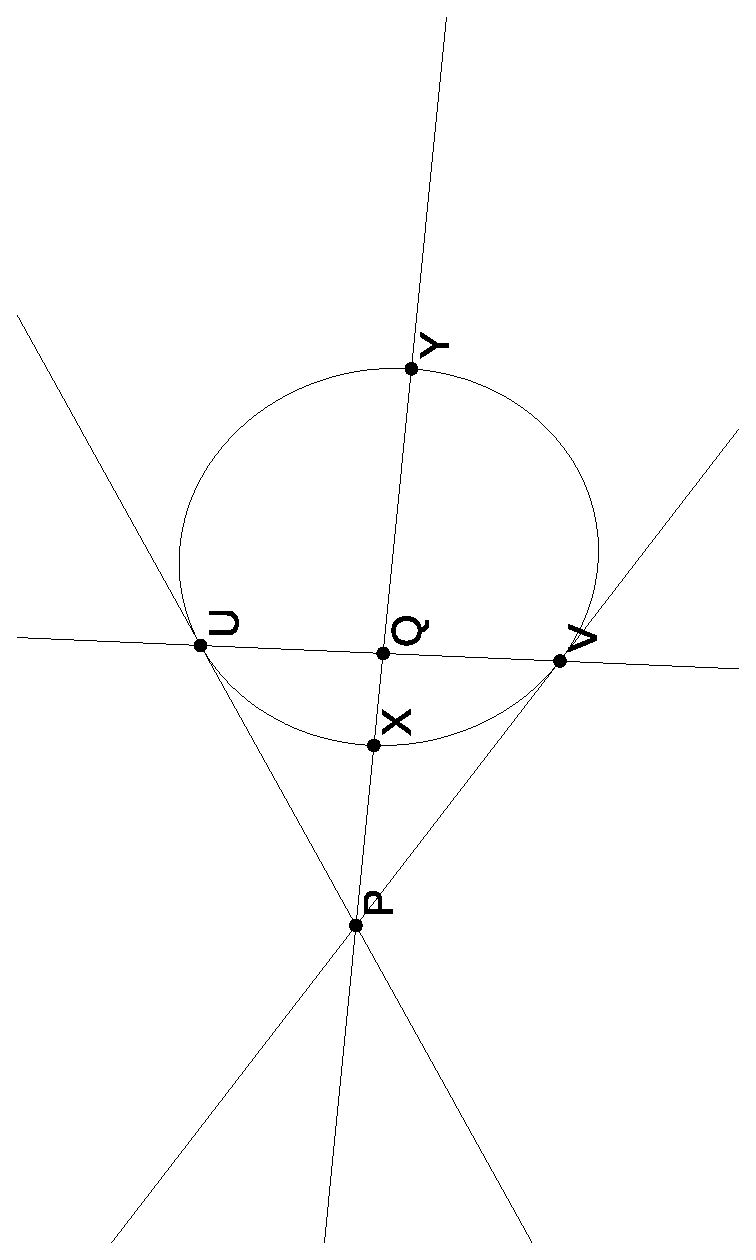
\includegraphics[scale=0.5,angle=270]{polartang.eps}
\caption{Proving $P,Q$ are conjugate}
\end{figure}

Chasing cross ratios, we have
\[
(P,Q;X,Y) \stackrel{U}{=} (U,V;X,Y)_\omega \stackrel{V}{=} (Q,P;X,Y),
\]
so $P,Q,X,Y$ are harmonic.
\end{proof}
\begin{proof}[Proof 2, using chords]
Let $AC$ and $BD$ be any two chords of $\omega$ passing through $P$. Let $E = AB\cap CD, F = AD\cap BC$. We will show that every point $Q$ on the line $EF$ is a harmonic conjugate of $P$ with respect to $\omega$. Let $AP\cap EF = R$, let $\omega$ meet $PQ$ at $X,Y$, and let $U = AB\cap PQ, V = CD\cap PQ$.

\begin{figure}[!htb]
\centering
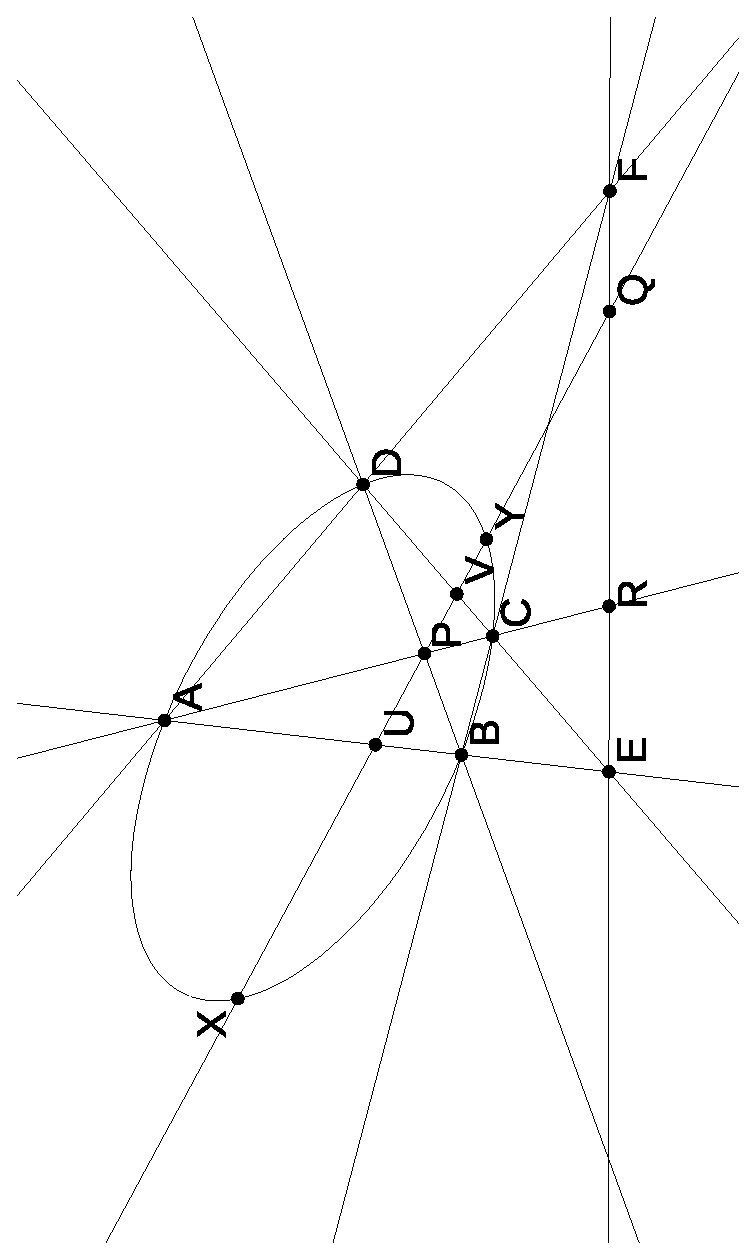
\includegraphics[scale=0.5,angle=270]{polar.eps}
\caption{Proving $P,Q$ are conjugate}
\end{figure}

By the quadrilateral theorem applied to the quadrilateral $BEDF$, the points $A,C,P,R$ are harmonic. Projecting through $E$, we see that the four points $U,V,P,Q$ are harmonic. Furthermore, by the projective butterfly theorem we have
\[
(X,Y;P,U) = (Y,X;P,V).
\]
Now suppose that $Q'$ is the harmonic conjugate of $P$ with respect to $X,Y$. Then if $h_{PQ'}$ denotes harmonic conjugation with respect to $P,Q'$ we have
\[
(X,Y;P,U) = (h_{PQ'}(X),h_{PQ'}(Y);h_{PQ'}(P),h_{PQ'}(U)) = (Y,X;P,h_{PQ'}(U)),
\]
so $h_{PQ'}(U) = V$. Thus $U,V,P,Q'$ are harmonic, so in fact we have $Q=Q'$.
\end{proof}

\begin{defn} If $P$ is a point, $\omega$ a conic, and $p$ is the locus of harmonic conjugates of $P$ with respect to $\omega$ then we say that $P$ is the \emph{pole} of the line $p$, and $p$ is the \emph{polar} of the point $P$. When several conics are around, we will usually write $\rho_\omega$ for the \emph{polar map} taking a point $P$ to its polar $p$ with respect to $\omega$ and taking a line $p$ to its pole $P$ with respect to $\omega$.
\end{defn}

\begin{prop} Every line $p$ has a unique pole $P$ with respect to $\omega$.
\end{prop}
\begin{proof} Let $Q,R$ be any two distinct points on $p$, and let their polars be $q, r$. Then $q,r$ intersect in at least one point $P$. By definition, $P$ is conjugate to $Q$ and $R$ with respect to $\omega$, so the polar of $P$ must be the line $QR = p$. Uniqueness is left as an exercise (consider the line joining two distinct poles of $p$).
\end{proof}

\begin{prop} Let $\omega$ be a conic, let $P,Q$ be points, and let $p,q$ be their polars with respect to $\omega$.
\begin{itemize}
\item[(a)] $P$ is on $q$ if and only if $Q$ is on $p$.
\item[(b)] $P$ is on $p$ if and only if $P$ is on $\omega$, in which case $p$ is tangent to $\omega$.
\item[(c)] If $X,Y$ are the feet of the tangent lines from $P$ to $\omega$, then $p = XY$.
\end{itemize}
\end{prop}
\begin{proof} The claims (a) and (b) are obvious from the definitions, while (c) follows easily from (a) and (b).
\end{proof}

\begin{prop} Let $\omega$ be a conic. The either $\omega$ is a parabola or $\omega$ is centrally symmetric around a point $O$. If $\omega$ is a hyperbola, then $O$ is the intersection of the asymptotes of $\omega$.
\end{prop}
\begin{proof} Let $O$ be the pole of the line at infinity. If $O$ is infinite, then $\omega$ must be tangent to the line at infinity at $O$, in which case $\omega$ is a parabola.

Now assume $O$ is finite. Then for any chord $X,Y$ through $O$, the points $X,Y,O,$ and the point at infinity along $XY$ are harmonic conjugates, so $O$ is the midpoint of $XY$, i.e. $\omega$ is centrally symmetric around $O$. If $\omega$ is a hyperbola, then the asymptotes intersect at the pole of the line at infinity, which is $O$ (this is still true if $\omega$ is an ellipse or a circle, but in that case the asymptotes have imaginary slopes).
\end{proof}

\begin{thm} Let $\omega$ be a circle with center $O$. Let $P\ne O$ be a finite point, and let $P'$ be its inverse with respect to the circle $\omega$. Then the polar of $P$ passes through $P'$ and is perpendicular to the line $OP$.
\end{thm}
\begin{proof} Let $\omega$ meet $OP$ in the points $X,Y$. When we restrict inversion to the line $OP$, we see that it is a nontrivial involution fixing $X$ and $Y$, so it must be harmonic conjugation with respect to $X,Y$. Thus $X,Y,P,P'$ are harmonic conjugates (this can also be checked using coordinates, or alternatively by drawing tangents and using facts we have already proven about harmonic quadrilaterals).

Now let $OP$ meet the line at infinity in the point $L$, and let $M$ be the harmonic conjugate of $L$ with respect to the circle points $\fish, \bar\fish$. Let $l, m, o, p$ denote the polars of $L, M, O, P$, respectively. Since the circle points are the intersection of $\omega$ with the line at infinity, $L$ and $M$ are conjugate with respect to $\omega$, so $M = o\cap l$ and thus $m = OL$. Since $P$ is on $m$, $M$ must be on $p$, so $p = MP'$. By the angle theorem, $MP'$ is perpendicular to $OP$, so we are done.
\end{proof}

\begin{thm}\label{polarcross} Let $\omega$ be a conic, and let points $A,B,C,D$ on a line $l$ have polars $a,b,c,d$. Then we have
\[
(A,B;C,D) = (a,b;c,d).
\]
\end{thm}
\begin{proof} Note that all four lines $a,b,c,d$ pass through $L$, the pole of $l$. First suppose that $l$ is not tangent to $\omega$. Let $\omega$ intersect $l$ in points $X,Y$, and let $a,b,c,d$ intersect $l$ at the points $A',B',C',D'$. Then by the definition of the polar, the points $A',B',C',D'$ are the harmonic conjugates of $A,B,C,D$ with respect to $X,Y$. Thus if $h_{XY}$ denotes harmonic conjugation with respect to $X,Y$, we have
\[
(A,B;C,D) = (h_{XY}(A),h_{XY}(B);h_{XY}(C),h_{XY}(D)) = (A',B';C',D') \stackrel{L}{=} (a,b;c,d).
\]

Now suppose the line $l$ is tangent to $\omega$. Let $M$ be any point not on $l$ or $\omega$, and let $m$ be its polar with respect to $\omega$. Then by the previous case applied to the line $m$,
\[
(A,B;C,D) = (MA,MB;MC,MD) = (m\cap a, m\cap b; m\cap c;, m\cap d) = (a,b;c,d).\qedhere
\]
\end{proof}

\begin{exer} Give a direct proof of Theorem \ref{polarcross} in the case that the line $l$ is tangent to $\omega$. (Hint: consider the map from $l$ to $\omega$ taking a point $P$ on $l$ to the foot of the second tangent from $P$ to $\omega$. Prove that this map preserves the cross ratio.)
\end{exer}

\begin{exer} Suppose $\omega_1, \omega_2$ are two conics which intersect at points $A, B, C, D$, and let $P = AB \cap CD$. Show that the the polar of $P$ with respect to $\omega_1$ and the polar of $P$ with respect to $\omega_2$ are the same.
\end{exer}

\begin{figure}[!htb]
\centering
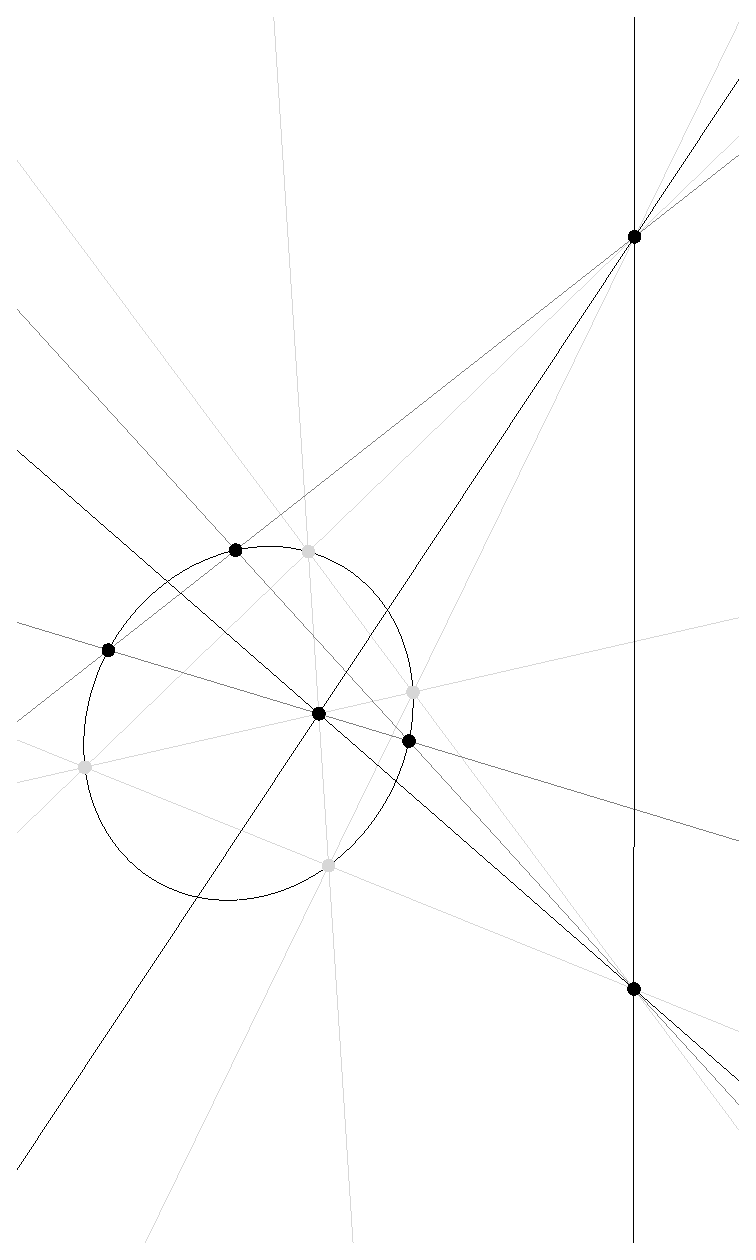
\includegraphics[scale=0.4,angle=270]{selfpolar.eps}
\caption{A self-polar triangle (Exercise \ref{selfpolar})}
\end{figure}

\begin{exer}\label{selfpolar}\hspace{2em}
\begin{itemize}
\item[(a)] Let $ABCD$ be a quadrilateral inscribed in a conic $\omega$. Let $E = AB\cap CD, F = AD\cap BC$ be the intersections of the opposite sides, and let $G = AC\cap BD$ be the intersection of the diagonals. Prove that the triangle $EFG$ is \emph{self-polar} with respect to $\omega$, that is, that the polars of $E,F,G$ are $FG,GE,EF$, respectively.

\item[(b)] Let $ABC$ be a self-polar triangle with respect to a conic $\omega$, and let $X,Y,Z$ be points on $\omega$ such that $Z,A,Y$ are collinear and $X,B,Z$ are collinear. Prove that $Y,C,X$ are collinear.
\end{itemize}
\end{exer}

\begin{exer} If $a,b,c,d,e$ are lines tangent to a conic $\omega$, define the cross ratio of $a,b,c,d$ with respect to $\omega$ by
\[
(a,b;c,d)_\omega = (a\cap e,b\cap e;c\cap e,d\cap e).
\]
\begin{itemize}
\item[(a)] Show that $(a,b;c,d)_\omega$ is independent of the choice of $e$.

\item[(b)] If $a,b,c,d$ meet $\omega$ at $A,B,C,D$, show that
\[
(a,b;c,d)_\omega = (A,B;C,D)_\omega.
\]
\end{itemize}
\end{exer}

\begin{exer}[Anders Kaseorg] Let $\omega, \Omega$ be distinct circles, and let $\rho_\omega, \rho_\Omega$ be the polar maps with respect to $\omega, \Omega$. Show that the composite map $\rho_\omega\circ\rho_\Omega\circ\rho_\omega\circ\rho_\Omega\circ\rho_\omega\circ\rho_\Omega$ is the identity if and only if the circles $\omega,\Omega$ have equal radii and intersect in $60^\circ$ arcs.
\end{exer}

\subsection{Coharmonic points}

For any two pairs of distinct points $\{A,X\}$ and $\{B,Y\}$ on a line, we can find a M\"obius transformation $f$ satisfying $f(A) = X$, $f(X) = A$, $f(B) = Y$ (since M\"obius transformations have three independent parameters). Since $f$ preserves the cross ratio, for any other point $C$ we must have
\[
(X,A;f(C),C) = (A,X;C,f(C)) = (f(A),f(X);f(C),f(f(C))) = (X,A;f(C),f(f(C))),
\]
so $C = f(f(C))$ and $f$ is a harmonic conjugation in a pair of points $\{M,N\}$. Motivated by this fact, we make the following definition.

\begin{defn} Three pairs of points $\{A,X\}, \{B,Y\}, \{C,Z\}$ on the same line are called \emph{coharmonic} if there is another pair of (possibly imaginary) points $\{M,N\}$ such that
\[
(M,N;A,X) = (M,N;B,Y) = (M,N;C,Z) = -1.
\]
\end{defn}

\begin{rem} Most geometers use the phrase ``quadrangular hexad'' to describe a collection of six coharmonic points.
\end{rem}

\begin{thm}[Main theorem of coharmonic points]\label{coharmonic} Let $A,B,C,X,Y,Z$ be on a line, no three the same, and suppose $A\ne X$. The following are equivalent:
\begin{itemize}
\item[\rm (a)] The three pairs of points $\{A,X\}, \{B,Y\}, \{C,Z\}$ are coharmonic.
\item[\rm (b)] There is a M\"obius transformation $f$ satisfying $f(A) = X, f(B) = Y, f(C) = Z$ which is an involution.
\item[\rm (c)] $(A,X;B,C) = (X,A;Y,Z)$.
\item[\rm (d)] $\frac{AY}{YC}\frac{CX}{XB}\frac{BZ}{ZA} = -1$.
\end{itemize}
\end{thm}
\begin{proof} By the above discussion, (a) and (b) are clearly equivalent. To see the equivalence of (b) and (c), let $f$ be the M\"obius function satisfying $f(A) = X, f(X) = A, f(B) = Y$. Then since $f$ preserves the cross ratio, we have
\[
(A,X;B,C) = (f(A),f(X);f(B),f(C)) = (X,A;Y,f(C)),
\]
so $f(C) = Z$ if and only if $(A,X;B,C) = (X,A;Y,Z)$.

Now we show that (b) implies (d). We start by making the definition
\[
(A,B,C;X,Y,Z) = \frac{AY}{YC}\frac{CX}{XB}\frac{BZ}{ZA}.
\]
This can also be written as
\[
(A,B,C;X,Y,Z) = -(A,C;Y,B)(B,A;Z,C)(C,B;X,A),
\]
so it is preserved by any M\"obius transformation. Thus
\[
(A,B,C;X,Y,Z) = (f(A),f(B),f(C);f(X),f(Y),f(Z)) = (X,Y,Z;A,B,C) = 1/(A,B,C;X,Y,Z),
\]
so $(A,B,C;X,Y,Z) = \pm 1$. To determine whether it is $1$ or $-1$, we need to work with coordinates. Since $(A,B,C;X,Y,Z)$ is a projective invariant, we can choose coordinates so that the fixed points of $f$ are $0$ and $\infty$. Then $f(z) = -z$ for any $z$. Let the coordinates of $A,B,C$ be $a,b,c$ so the coordinates of $X,Y,Z$ are $-a, -b, -c$. Then
\[
(A,B,C;X,Y,Z) = \frac{a+b}{-b-c}\cdot\frac{c+a}{-a-b}\cdot\frac{b+c}{-c-a} = -1.
\]
Finally, to see that (d) implies (b), note that for any $A,B,C,X,Y$ there is a unique $Z$ such that $(A,B,C;X,Y,Z) = -1$, and if $f$ is a M\"obius involution taking $A$ to $X$ and $B$ to $Y$, then $(A,B,C;X,Y,f(C)) = -1$ by the above.
\end{proof}

\begin{thm}[Three Conic Law] Let $A,B,C,D$ be any four points, no three on a line. Let $l$ be a line passing through at most one of $A,B,C,D$. Let $\omega_1,\omega_2,\omega_3$ be three (possibly degenerate) conics passing through $A,B,C,D$. For each $i=1,2,3$, let $X_i, Y_i$ be the two points of intersection of conic $\omega_i$ with line $l$. Then the three pairs $\{X_1, Y_1\}, \{X_2,Y_2\}, \{X_3,Y_3\}$ are coharmonic.
\end{thm}
\begin{proof} Consider the following map $f$ from the line $l$ to itself. For any point $P$ on $l$, let $\omega_P$ be the conic passing through the points $A,B,C,D,P$, and define $f(P)$ to be the second point of intersection of $\omega_P$ with the line $l$. By Theorem \ref{invariant}, or more concretely by the solution to Exercise \ref{conicline}, $f$ is a M\"obius transformation. Since $f$ is clearly also an involution satisfying $f(X_i) = Y_i$ for $i=1,2,3$, the main theorem of coharmonic points shows that $\{X_1, Y_1\}, \{X_2,Y_2\}, \{X_3,Y_3\}$ are coharmonic.
\end{proof}

\begin{figure}[!htb]
\centering
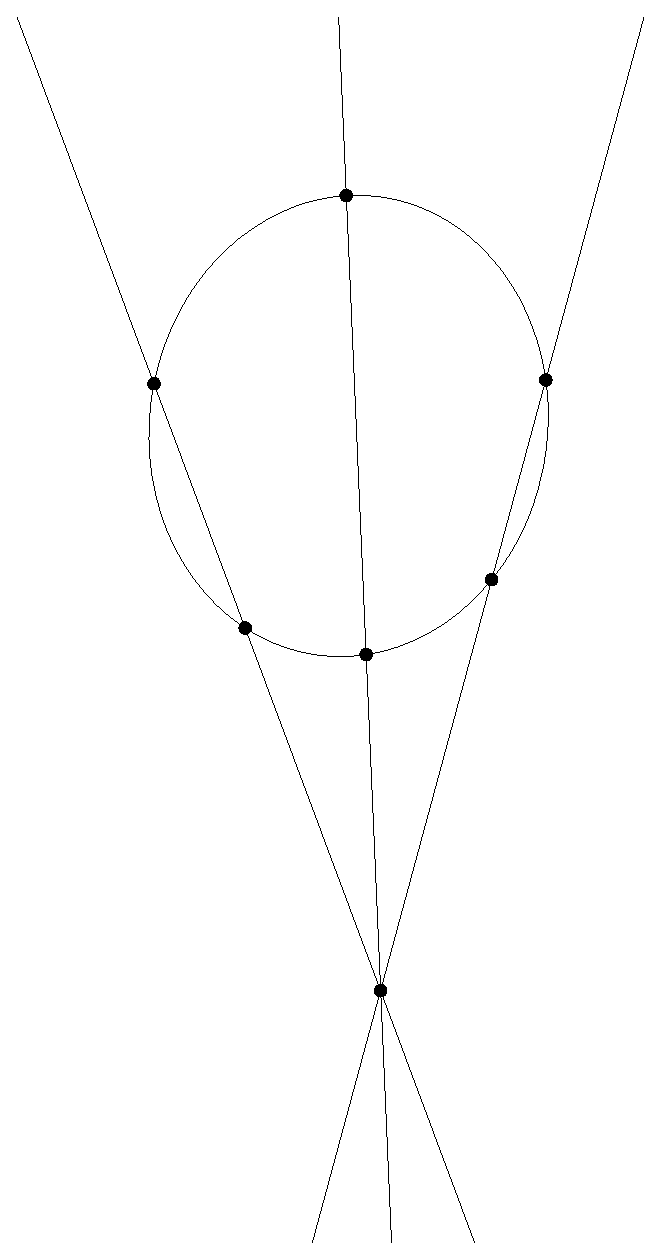
\includegraphics[scale=0.3,angle=270]{coharmonic.eps}
\caption{Coharmonic points on a conic}\label{coharmonic-conic}
\end{figure}

\begin{exer}
\begin{itemize}
\item[(a)] Let $\omega$ be a conic, and let $P$ be a point not on $\omega$, and let $A,B,C$ be three points on $\omega$. Let $X,Y,Z$ be the second intersections of the lines $PA,PB,PC$ with $\omega$. Show that the three pairs $\{A,X\}, \{B,Y\}, \{C,Z\}$ are coharmonic with respect to the conic $\omega$. (Hint: see Exercise 5.)
\item[(b)] Suppose that $ABCDEF$ is a convex hexagon inscribed in a circle $\omega$. Show, using part (a), that the lines $AD, BE, CF$ meet in a point if and only if
\[
|AB||CD||EF| = |BC||DE||FA|.
\]
(Hint: define $(A,E,C;D,B,F)_{\omega}$ for any conic $\omega$, and calculate it in the special case that $\omega$ is a circle.) How is this related to the trigonometric form of Ceva's Theorem?
\end{itemize}
\end{exer}

\begin{exer} Suppose that $A,B,C,X,Y,Z$ are six points on a conic $\omega$. Let $U$ be the intersection between the line $BC$ and the tangent to $\omega$ at $X$, and similarly let $V$ be the intersection between $AC$ and the tangent to $\omega$ at $Y$, and $W$ the intersection between $AB$ and the tangent to $\omega$ at $Z$. Show that if $\{A,X\},\{B,Y\},\{C,Z\}$ are coharmonic with respect to $\omega$, then $U,V,W$ are collinear. Is the converse true?
\end{exer}

\begin{exer} Apply the Three Conic Law to give a second proof of the projective Butterfly Theorem: if $\omega$ is a conic, $PQ$ is a chord on $\omega$, $M$ is a point on $PQ$, $AB$ and $CD$ are two more chords of $\omega$ passing through $M$, and $X = AD\cap PQ, Y = BC\cap PQ$, then $(P,Q;M,X) = (Q,P;M,Y)$. (Hint: show that $\{P,Q\}, \{M,M\}, \{X,Y\}$ are coharmonic.)
\end{exer}

\begin{exer} Apply a degenerate case of the Three Conic Law to give a second proof of the Quadrilateral Theorem. (Hint: what does it mean for $\{X,Y\},\{E,E\},\{F,F\}$ to be coharmonic?)
\end{exer}

\begin{exer} Apply the Three Conic Law to give a second proof of Desargues' Theorem. (Hint: In the notation of Theorem \ref{desargues}, show that $\{PA\cap VW,BC\cap VW\},\{PB\cap VW, V\}, \{PC\cap VW,W\}$ are coharmonic, and compare the corresponding statement with $A,B,C$ replaced by $X,Y,Z$.)
\end{exer}

\begin{exer} Let $\omega, \Omega$ be a pair of circles intersecting at points $A,B$, and let $P$ be a point on the line $AB$. Let $l$ be a line through $P$, let $X,Y$ be the points of intersection between $l$ and $\omega$, and let $U,V$ be the points of intersection between $l$ and $\Omega$. Show that
\[
PX\cdot PY = PU\cdot PV.
\]
\end{exer}

\begin{exer} Let $A,B,C,D,E$ lie on a conic $\omega$, and let $l$ be a line which is tangent to $\omega$ at $E$. Construct, using only a straightedge, the point $F \ne E$ on $l$ such that the conic $\omega'$ passing through $A,B,C,D,F$ is tangent to the line $l$ at $F$.
\end{exer}

\begin{figure}[!htb]
\centering
\includegraphics[scale=0.5,angle=270]{octa.eps}
\caption{Octagrammum Mysticum}\label{octa}
\end{figure}

\begin{thm}[Octagrammum Mysticum] Let $A,B,C,D,E,F,G,H$ be eight points, no three on a line. Let $I = GH\cap BC, J = HA\cap CD, K = AB\cap DE$, etc., as in Figure \ref{octa}. Then $A,B,C,D,E,F,G,H$ lie on a conic if and only if $I,J,K,L,M,N,O,P$ lie on a conic.
\end{thm}
\begin{proof}[Proof 1 (using coharmonicity)] Suppose that $I,J,K,L,M,N,O,P$ lie on a conic $\omega$. It's enough to show that $(AF,AD;AH,AB) = (J,P;L,N)_\omega$, since then by symmetry we will have
\[
(J,P;L,N)_\omega = (CF,CD;CH,CB) = (EF,ED;EH,EB) = (GF,GD;GH,GB),
\]
from which we can conclude that $C,E,G$ are on the conic through $A,F,D,H,B$. To this end, we project everything onto the line $DF$.
\begin{figure}[!htb]
\centering
\includegraphics[scale=0.5,angle=270]{octa1.eps}
\caption{Proving $(AF,AD;AH,AB) = (J,P;L,N)_\omega$}\label{octa1}
\end{figure}
Let $S = AB \cap DF, T = AH \cap DF, U = ML \cap DF, V = MN \cap DF$, and let $X,Y$ be the (possibly imaginary) points of intersection between $\omega$ and $DF$. We have
\[
(AF,AD;AH,AB) = (F,D;T,S)
\]
and
\[
(J,P;L,N)_\omega \stackrel{M}{=} (D,F;U,V),
\]
so by Theorem \ref{coharmonic} it's enough to show that $\{D,F\},\{U,T\},\{S,V\}$ are coharmonic.

Applying Three Conic Law to the points $M,L,J,O$, the line $DF$, the conic $\omega$ and the degenerate conics $ML\cup JO, MJ\cup LO$, we see that $\{D,F\}, \{X,Y\}, \{U,T\}$ are coharmonic. Similarly, applying the Three Conic Law to the points $M,N,K,P$, the line $DF$, the conic $\omega$ and the conics $MN\cup KP, MP\cup NK$, we see that $\{D,F\}, \{X,Y\}, \{S,V\}$ are coharmonic.

Thus the harmonic conjugation map that exchanges $D$ with $F$ and exchanges $X$ with $Y$ also exchanges $U$ with $T$ and $S$ with $V$, so $\{D,F\},\{U,T\},\{S,V\}$ are coharmonic and we are done.
\end{proof}
\begin{proof}[Proof 2 (from \cite{mystic}, using Pascal's Theorem)] Again, we assume that $I,J,K,L,M,N,O,P$ lie on a conic $\omega$. It's enough to show that $G,H,A,B,C,D$ lie on a conic, since then by symmetry we have $H,A,B,C,D,E$ on a conic, etc.

Let $X$ be the intersection of lines $KP$ and $IJ$. Applying Pascal's Theorem to the hexagon $MPKNIJ$ inscribed in the conic $\omega$, we see that $D, G, X$ lie on a line. From this we see that $I, J, X$ are the intersections of the opposite sides of the hexagon $GHABCD$, so by the converse to Pascal's Theorem $GHABCD$ is also inscribed in a conic.
\begin{figure}[!htb]
\centering
\includegraphics[scale=0.5,angle=270]{octa2.eps}
\caption{Applying Pascal}\label{octa2}
\end{figure}
\end{proof}

\subsection{Symmetries of the plane}

\begin{defn} Let $M = \left(\begin{array}{ccc}a & b & c\\ d & e & f\\ g & h & i\end{array}\right)$ be a three by three matrix with nonzero determinant. The map $f_M:\PP^2\rightarrow \PP^2$ defined by $f([x:y:z]) = [ax+by+cz:dx+ey+fz:gx+hy+iz]$ is called a \emph{projective transformation} of the plane.
\end{defn}

\begin{exer}\label{projective-trans}\hspace{2em}
\begin{itemize}
\item[(a)] Show that every projective transformation sends straight lines to straight lines, sends conics to conics, and preserves cross ratios.

\item[(b)] Show that if $M,N$ are three by three matrices with nonzero determinants, then $f_M\circ f_N = f_{MN}$.

\item[(c)] Show that if $A,B,C,D$ are any four points with no three on a line, and $E,F,G,H$ are any four points with no three on a line, then there is a projective transformation $f$ with $f(A) = E, f(B) = F, f(C) = G, f(D) = H$.
\end{itemize}
\end{exer}

\begin{defn} A bijection $f:\PP^2 \rightarrow \PP^2$ is a \emph{collineation} if it takes straight lines to straight lines.
\end{defn}

\begin{exer}\label{cr-arithmetic}\hspace{2em}
\begin{itemize}
\item[(a)] Let $A,B,C,D,E,F$ be six distinct points on a line. Show that $\{A,B\},\{C,D\},\{E,F\}$ are coharmonic if and only if
\[
(A,B;C,D) = (A,B;C,E)(A,B;C,F).
\]

\item[(b)] Given distinct points $A,B,C,D,E$ on a line, construct points $F$ and $G$ on the same line such that
\[
(A,B;C,F) = (A,B;C,D)(A,B;C,E)
\]
and
\[
(A,B;C,G) = (A,B;C,D) + (A,B;C,E)
\]
using only a straightedge.
\end{itemize}
\end{exer}

\begin{exer}\label{rigid-R} Let $f:\RR\rightarrow\RR$ be a function such that $f(1) = 1$ and such that for any $x,y \in \RR$ we have $f(xy) = f(x)f(y)$ and $f(x+y) = f(x)+f(y)$. Show that $f(x) = x$ for all $x\in \RR$.
\end{exer}

\begin{thm}[Fundamental theorem of projective geometry] A bijection $f:\RR\PP^2 \rightarrow \RR\PP^2$ is a collineation if and only if it is a projective transformation (here we write $\RR\PP^2$ for the \emph{real} points of the projective plane).
\end{thm}
\begin{proof} We start by showing that if $f$ is a collineation then it must preserve cross ratios. If $A,B,C,D$ are distinct points on a line and $E,F,G,H$ are distinct points on another line, then by Theorem \ref{cr-equal} we can check whether $(A,B;C,D) = (E,F;G,H)$ by checking whether the points $X = AF\cap BE, Y = BG\cap CF, Z = CH\cap DG$ lie on a line. Since $f$ is a collineation, we have $f(X) = f(AF)\cap f(BE) = f(A)f(F)\cap f(B)f(E)$ and so on, and $f(X), f(Y), f(Z)$ lie on a line if and only if $X,Y,Z$ lie on a line, so
\[
(A,B;C,D) = (E,F;G,H) \iff (f(A),f(B);f(C),f(D)) = (f(E),f(F);f(G),f(H)).
\]
Thus we get a well-defined bijection $\tilde{f}:\RR\cup\{\infty\}\rightarrow\RR\cup\{\infty\}$ by taking
\[
\tilde{f}((A,B;C,D)) = (f(A),f(B);f(C),f(D)).
\]
This bijection automatically satisfies $\tilde{f}(0) = 0, \tilde{f}(1) = 1, \tilde{f}(\infty) = \infty$. By Exercise \ref{cr-arithmetic} we have $\tilde{f}(xy) = \tilde{f}(x)\tilde{f}(y)$ and $\tilde{f}(x+y) = \tilde{f}(x)+\tilde{f}(y)$ for any real $x,y$, and thus by Exercise \ref{rigid-R} we must have $\tilde{f}(x) = x$ for all real $x$. Thus $f$ preserves cross ratios.

To finish, note that by Exercise \ref{projective-trans} we may assume without loss of generality that $f$ fixes some collection of four points $A,B,C,D$ such that no three are on a line. Letting $P = AB\cap CD$, we see that $f(P) = P$, and thus for any point $X$ on $AB$ we have
\[
(A,B;P,X) = (f(A),f(B);f(P),f(X)) = (A,B;P,f(X)),
\]
so $f(X) = X$. Thus if $l$ is any line through $C$, and $X = l \cap AB$, then $f(l) = f(C)f(X) = CX = l$, so every line through $C$ is sent to itself. Similarly, every line through $A$ or $B$ is sent to itself. Since any point $E$ is determined by the three lines $AE,BE,CE$, every point $E$ must be sent to itself, and we are done.
\end{proof}

\begin{rem} A collineation of $\CC\PP^2$ might not preserve cross ratios: for instance, the map $[x:y:z] \mapsto [\bar{x}:\bar{y}:\bar{z}]$ taking every point to its complex conjugate sends every cross ratio to its complex conjugate. More generally, if $\tilde{f}:\CC\rightarrow\CC$ satisfies $\tilde{f}(1) = 1, \tilde{f}(xy) = \tilde{f}(x)\tilde{f}(y), \tilde{f}(x+y) = \tilde{f}(x)+\tilde{f}(y)$, then the map $[x:y:z] \mapsto [\tilde{f}(x):\tilde{f}(y):\tilde{f}(z)]$ is called an \emph{automorphic collineation}, and sends a set of four points on a line with cross ratio $c$ to a set of four points with cross ratio $\tilde{f}(c)$.

The same argument as above can be used to show that every collineation of $\CC\PP^2$ can be written as the composition of an automorphic collineation and a projective transformation.
\end{rem}

\begin{defn} Let $P$ be a point and $l$ be a line not passing through $P$. Define the \emph{projective reflection} $r_{P,l}$ by sending a point $Q \ne P$ to the harmonic conjugate of $Q$ with respect to $P, PQ \cap l$ along the line $PQ$, and sending $P$ to $P$.
\end{defn}

\begin{ex}
\begin{itemize}
\item[(a)] Let $l$ intersect the line at infinity at $L$. If $P$ is on the line at infinity with $L,P,\fish,\bar\fish$ harmonic, then $r_{P,l}$ is (ordinary) reflection across the line $l$. As a consequence, (ordinary) reflections always interchange the two circle points.

\item[(b)] If $l$ is the line at infinity, then $r_{P,l}$ is a $180^\circ$ rotation around $P$ (sometimes called a reflection through the point $P$).
\end{itemize}
\end{ex}

\begin{thm} For any point $P$ and any line $l$ not passing through $P$, the projective reflection $r_{P,l}$ is a projective transformation.
\end{thm}
\begin{proof} We just need to show that $r_{P,l}$ sends lines to lines and preserves cross ratios. We leave this as an easy exercise to the reader.
\end{proof}

\begin{defn} If $A,B,C,D$ are four points with no three on a line and $\sigma:\{A,B,C,D\} \rightarrow \{A,B,C,D\}$ is a permutation, define $r_{\sigma}$ to be the projective transformation taking $A$ to $\sigma(A)$, $B$ to $\sigma(B)$, etc. We will often write $\sigma$ using its cycle decomposition, including the cycles of length $1$, so that for instance $r_{(A)(B)(C\;D)}$ is the projective transformation taking $A$ and $B$ to themselves, and swapping $C$ and $D$.
\end{defn}

\begin{exer} Suppose $A,B,C,D$ are four points with no three on a line.
\begin{itemize}
\item[(a)] If $P = AB\cap CD$ and $l$ is the line connecting $AC\cap BD$ to $AD\cap BC$, show that $r_{(A\;B)(C\;D)}$ is the projective reflection $r_{P,l}$.

\item[(b)] Show that if $\omega$ is a conic passing through $A,B,C,D$ then $r_{(A\;B)(C\;D)}(\omega) = \omega$.

\item[(c)] Show that if $\omega$ is as in (b) and $P,l$ are as in (a), then $l$ is the polar of $P$ with respect to $\omega$.
\end{itemize}
\end{exer}

\begin{exer}
\begin{itemize}
\item[(a)] Show that for every permutation $\sigma:\{A,B,C,D\} \rightarrow \{A,B,C,D\}$ we can write $r_\sigma$ as a composition of two projective reflections.

\item[(b)] Show that a projective transformation defined by a three by three matrix $M$ can be written as a composition of two projective reflections if and only if the eigenvalues of $M$ are in a geometric progression. % is this actually true when M has jordan blocks?
\end{itemize}
\end{exer}

\begin{exer} Let $f(p,q,r),g(p,q,r),h(p,q,r)$ be homogeneous polynomials of the same degree having no common factor. The map $[p:q:r]\mapsto [f(p,q,r):g(p,q,r):h(p,q,r)]$ is called \emph{biregular} if it is defined everywhere (i.e. $f,g,h$ are never simultaneously $0$ unless $p,q,r$ are all $0$) and is a bijection of the complex points of the projective plane. Prove that every biregular map is a projective transformation.
\end{exer}

% central collineations, homologies, elations?

One rather boring way to use symmetries of the plane is to choose a coordinate system in which four points $A,B,C,D$ in general position are assigned the coordinates $[1:0:0], [0:1:0], [0:0:1], [1:1:1]$. If a geometric configuration is completely determined by the locations of five points $A,B,C,D,E$, then every other point has coordinates given by homogenous algebraic functions of the coordinates $[x:y:z]$ of the point $E$. Problems involving such configurations can then be straightforwardly transformed into simple algebra problems, which typically will state that if one homogenous polynomial of the coordinates $[x:y:z]$ of $E$ vanishes, then so does another (often these polynomials will be linear or quadratic). Many problems in triangle geometry have this form: the five relevant points are the vertices $A,B,C$ of the triangle, and the two circle points $\fish$ and $\bar\fish$.

\begin{thm} If $A,B,C,D,E$ are five points in general position, and if we choose a coordinate system where $A,B,C,D,E$ are assigned the coordinates $[1:0:0], [0:1:0], [0:0:1], [1:1:1], [x:y:z]$, respectively, then we have
\[
\frac{y}{z} = (AB,AC;AD,AE)
\]
and
\[
\frac{x}{z} = (BA,BC;BD,BE).
\]
In particular, the pair of values of these two cross ratios completely determines which statements of projective geometry are true of the configuration $ABCDE$.
\end{thm}
\begin{proof} We will only prove the first equality, the second one is similar. We have
\begin{align*}
(AB,AC;AD,AE) &= (B,C;AD\cap BC, AE\cap BC)\\
&= ([0:1:0],[0:0:1];[0:1:1],[0:y:z]) = (\infty,0;1,y/z) = y/z.\qedhere
\end{align*}
\end{proof}

In the special case where $A,B,C$ are the vertices of a triangle and $D,E$ are the circle points $\fish,\bar\fish$, the previous theorem becomes the statement that every triangle $ABC$ is determined up to direct similarity by the ordered pair of directed angles $\angle BAC$ and $\angle ABC$ modulo $\pi$. So for instance, the correct projective generalization of the concept of an isosceles triangle is a configuration of five points $ABCDE$, no three on a line, which satisfies the symmetry
\[
r_{(A\;B)(D\;E)}(C) = C,
\]
and the projective analogue of an equilateral triangle will additionally satisfy the symmetry
\[
r_{(A\;C)(D\;E)}(B) = B.
\]

\begin{exer} Show that if no three of $A,B,C,D,E$ are on a line, and if the configuration $ABCDE$ satisfies the symmetries $r_{(A\;B)(D\;E)}(C) = C$ and $r_{(A\;C)(D\;E)}(B) = B$, then it also satisfies the symmetry $r_{(B\;C)(D\;E)}(A) = A$. Show that in this case, the cross ratio $(EA,EB;EC,ED)$ is \emph{melodic} in the sense of Exercise \ref{melodic}.
\end{exer}

\begin{exer} Show that if no three of $A,B,C,D,E$ are on a line, and if the configuration $ABCDE$ satisfies the symmetries $r_{(B\;E)(C\;D)}(A) = A$ and $r_{(A\;C)(D\;E)}(B) = B$, then it also satisfies the symmetry $r_{(A\;E)(B\;D)}(C) = C$. Show that in this case, the cross ratio $(EA,EB;EC,ED)$ is either the golden ratio $\phi$ or its algebraic conjugate $-1/\phi$.
\end{exer}

\subsection{The Cross Cross Ratio}

Since any four points (no three on a line) can be sent to any other four points (no three on a line) by a projective transformation, there are no interesting invariants of four general points in the plane. If we have five general points $A,B,C,D,E$, then we can form the cross ratio $(EA,EB;EC,ED)$. Going one step further, we have the following natural definition.

\begin{defn} Let $A,B,C,D,E,F$ be six points in the plane, such that either none of $ACE, ADF$, $BCF, BDE$ are lines or none of $ACF, ADE$, $BCE, BDF$ are lines. Define their \emph{cross cross ratio} to be
\[
(A,B;C,D;E,F) = \frac{(EA,EB;EC,ED)}{(FA,FB;FC,FD)}.
\]
\end{defn}

First we will prove that this definition is more symmetric than it seems.

\begin{figure}[!htb]
\centering
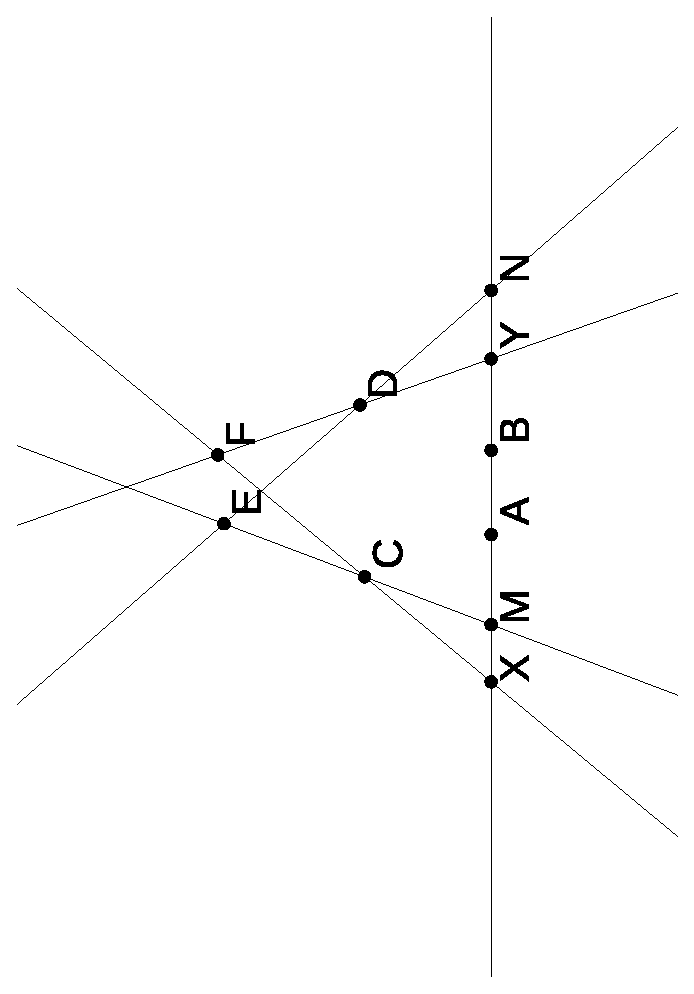
\includegraphics[scale=0.5,angle=270]{ccr.eps}
\caption{Symmetry of the cross cross ratio}
\end{figure}

\begin{thm} Let $A,B,C,D,E,F$ be as above. Then we have
\[
(A,B;C,D;E,F) = (A,B;E,F;C,D).
\]
\end{thm}
\begin{proof} We start by projecting everything onto the line $AB$. Let $M = EC\cap AB, N = ED\cap AB, X = FC\cap AB, Y = FD\cap AB$. Then we have
\begin{align*}
(A,B;C,D;E,F) &= \frac{(EA,EB;EC,ED)}{(FA,FB;FC,FD)} = \frac{(A,B;M,N)}{(A,B;X,Y)}\\
&= \frac{(A,B;M)}{(A,B;N)}\bigg/\frac{(A,B;X)}{(A,B;Y)} = \frac{(A,B;M)}{(A,B;X)}\bigg/\frac{(A,B;N)}{(A,B;Y)}\\
&= \frac{(A,B;M,X)}{(A,B;N,Y)} = \frac{(CA,CB;CE,CF)}{(DA,DB;DE,DF)} = (A,B;E,F;C,D).\qedhere
\end{align*}
\end{proof}

\begin{prop} Let two circles $\omega, \omega'$ intersect at points $A,B$, and let $C$ be a point on $\omega$, $D$ a point on $\omega'$. Let $\theta$ be the (directed) angle of intersection between the circles $\omega, \omega'$ at $A$. Then we have
\[
(A,B;\fish,\bar\fish;C,D) = e^{2i\theta}.
\]
In particular, $\omega$ and $\omega'$ are orthogonal if and only if $(A,B;\fish,\bar\fish;C,D) = -1$.
\end{prop}
\begin{proof}
\[
(A,B;\fish,\bar\fish;C,D) = \frac{(A,B;\fish,\bar\fish)_\omega}{(A,B;\fish,\bar\fish)_{\omega'}} = e^{2i(\angle ACB - \angle ADB)} = e^{2i\theta}.\qedhere
\]
\end{proof}

\begin{defn} If conics $\omega,\omega'$ meet in points $A,B,C,D$, set
\[
(A,B;C,D;\omega,\omega') = \frac{(A,B;C,D)_\omega}{(A,B;C,D)_{\omega'}}.
\]
If $(A,B;C,D;\omega,\omega') = -1$, we say that the conics $\omega, \omega'$ are \emph{projectively orthogonal with respect to the partition} $\{A,B\},\{C,D\}$ of their intersection points.
\end{defn}

\begin{figure}[!htb]
\centering
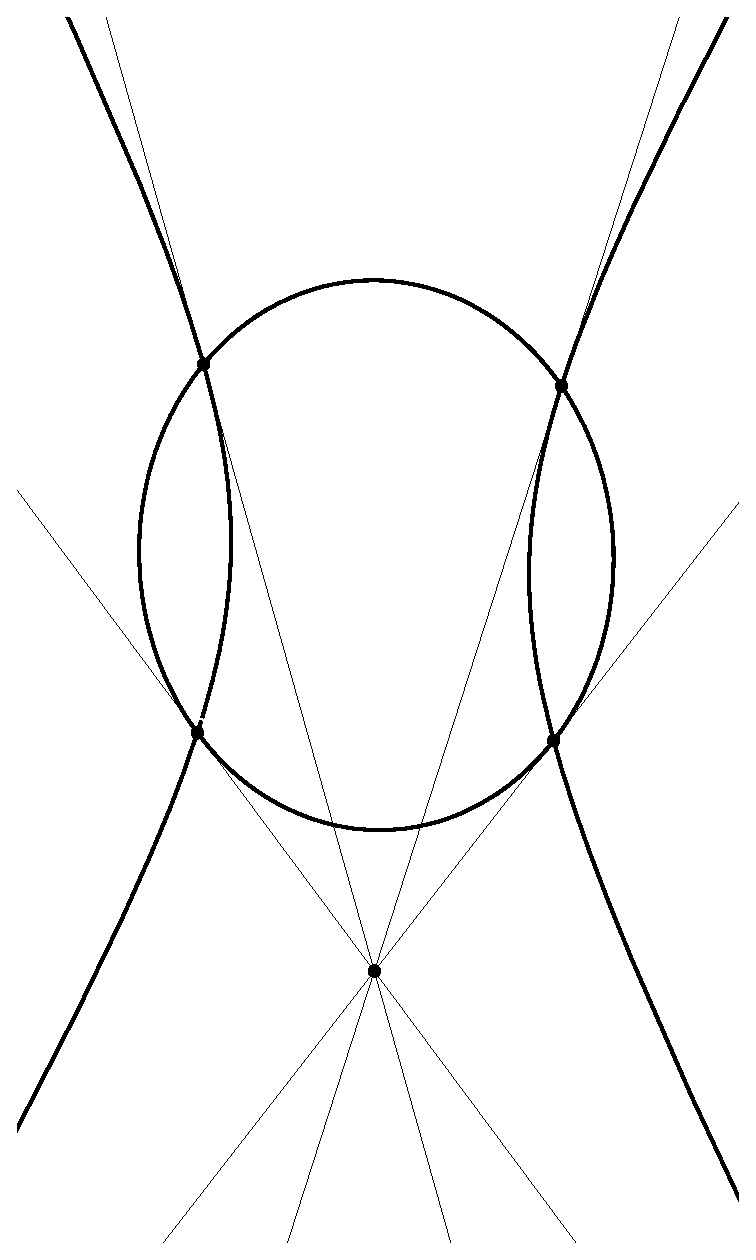
\includegraphics[scale=0.5,angle=270]{orthogonal.eps}
\caption{Projectively orthogonal conics}
\end{figure}

\begin{thm} Two conics $\omega, \Omega$ meeting in points $A,B,C,D$ are projectively orthogonal with respect to the partition $\{A,B\},\{C,D\}$ if and only if the two tangents to $\omega$ at $A$ and $B$ meet the two tangents to $\Omega$ at $C$ and $D$.
\end{thm}
\begin{proof} Let $E = AC\cap BD, F = AD\cap BC$. We will project everything onto the line $EF$: let $X = AB\cap EF$, let $Y = CD\cap EF$, let $P$ be the intersection of the tangent to $\omega$ at $A$ with $EF$, and let $Q$ be the intersection of the tangent to $\Omega$ at $C$ with $EF$.

\begin{figure}[!htb]
\centering
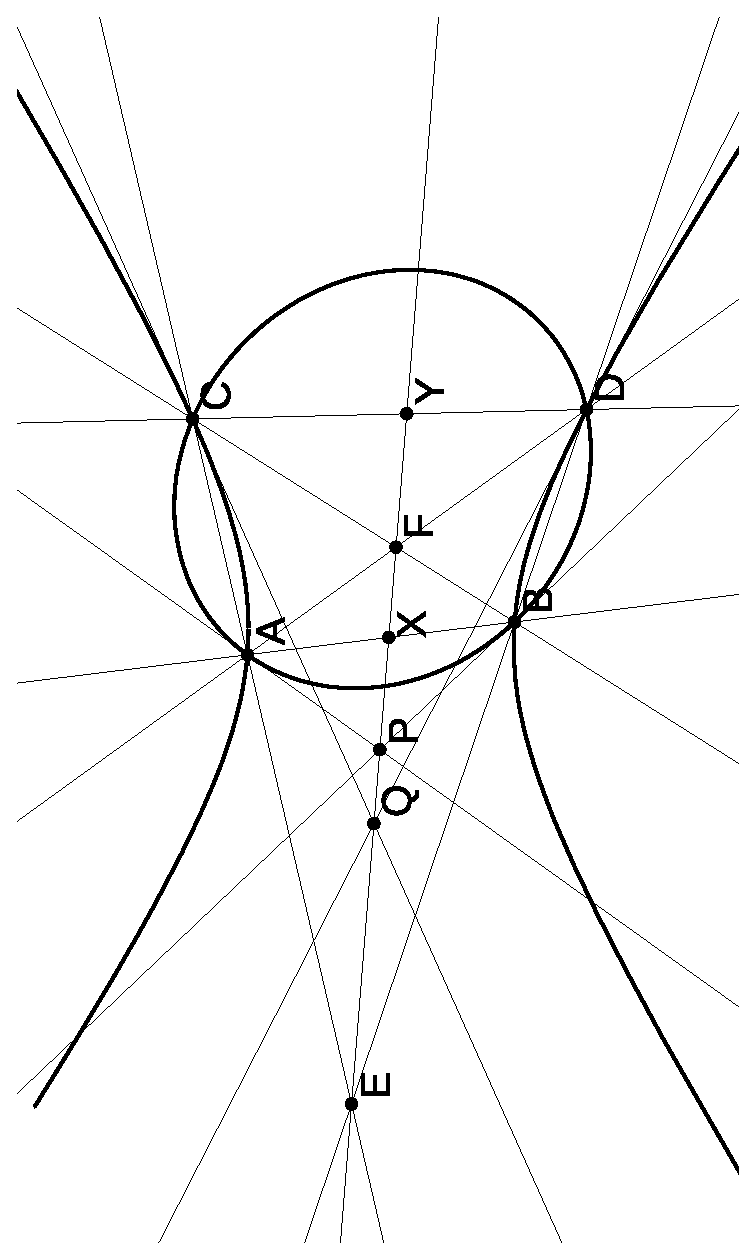
\includegraphics[scale=0.5,angle=270]{north.eps}
\caption{Checking orthogonality}
\end{figure}

Projecting through $A$ or $B$, we have
\[
(A,B;C,D)_\omega \stackrel{A}{=} (P,X;E,F) \stackrel{B}{=} (BP\cap\omega,A;D,C)_\omega,
\]
so $BP$ is also tangent to $\omega$, and similarly we have
\[
(A,B;C,D)_\Omega \stackrel{C}{=} (E,F;Q,Y) \stackrel{D}{=} (B,A;DQ\cap\Omega,C)_\Omega
\]
and $DQ$ is tangent to $\Omega$. By the quadrilateral theorem, we have
\[
(E,F;X,Y) = -1,
\]
so
\[
\frac{(A,B;C,D)_\omega}{(A,B;C,D)_\Omega} = \frac{(E,F;P,X)}{(E,F;Q,Y)} = \frac{(E,F;P,Q)}{(E,F;X,Y)} = -(E,F;P,Q).
\]
Thus $(A,B;C,D;\omega,\Omega) = -1$ if and only if $P = Q$.
\end{proof}

\begin{figure}[!htb]
\centering
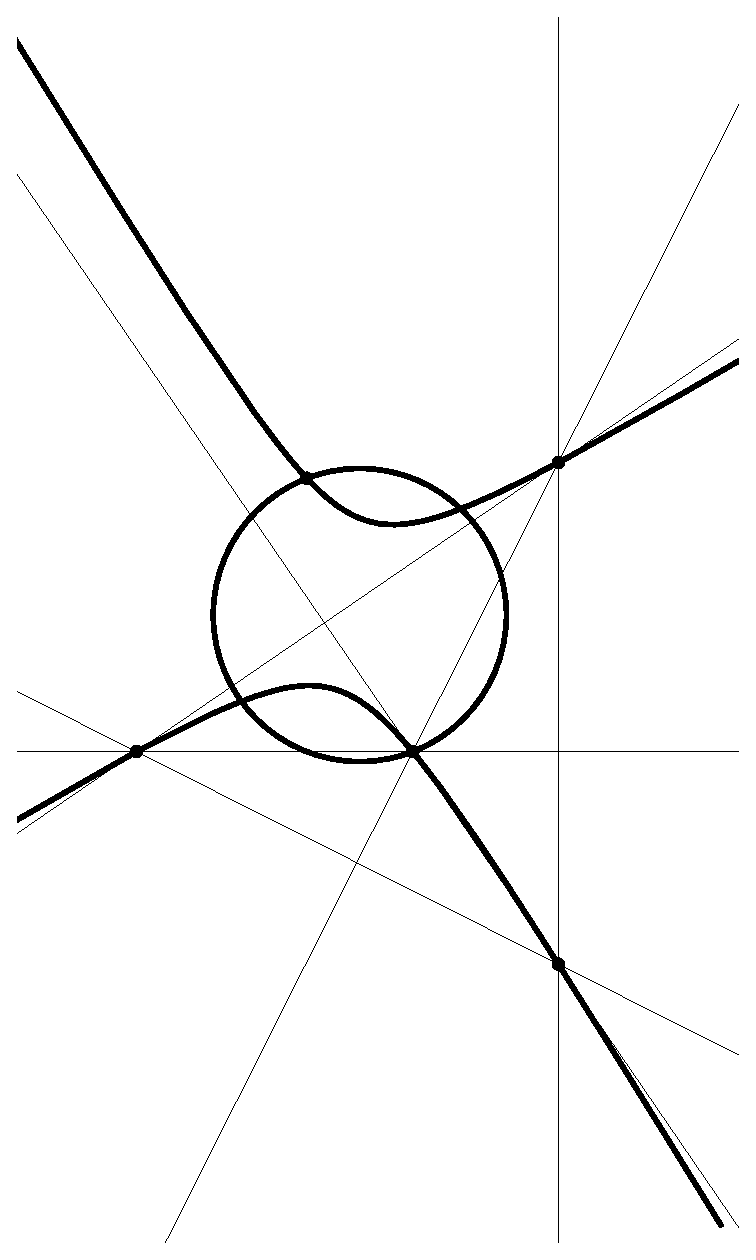
\includegraphics[scale=0.5,angle=270]{righthyperbola.eps}
\caption{Exercise \ref{orthohyperbola}}\label{righthyperbola}
\end{figure}

\begin{exer}\label{orthohyperbola} Let $H$ be the orthocenter of triangle $ABC$, and let $P$ be any point other than $H$. Let $\omega$ be the circle with diameter $HP$, and let $\Omega$ be the conic through $A,B,C,H,P$.
\begin{itemize}
\item[(a)] Show that the asymptotes to $\Omega$ meet at a right angle.

\item[(b)] Show that if $\omega$, $\Omega$ also meet at points $X,Y$, then $\omega$ is projectively orthogonal to $\Omega$ with respect to the partition $\{H,P\},\{X,Y\}$.
\end{itemize}
\end{exer}

\begin{exer} Suppose conics $\omega,\Omega$ meet at $A,B,C,D$ and are projectively orthogonal with respect to the partition $\{A,B\},\{C,D\}$ of their intersection points. Let $l$ be a line meeting $\omega$ at $P,Q$ and meeting $\Omega$ at $R,S$.
\begin{itemize}
\item[(a)] Show that $(P,Q;A,B)_\omega = -1$ if and only if $(R,S;C,D)_{\Omega} = -1$.

\item[(b)] Show that if $(P,Q;A,B)_\omega = -1$ then $(P,Q;R,S) = -1$.
\end{itemize}
\end{exer}

\subsection{A few miscellaneous exercises}

\begin{figure}[!htb]
\centering
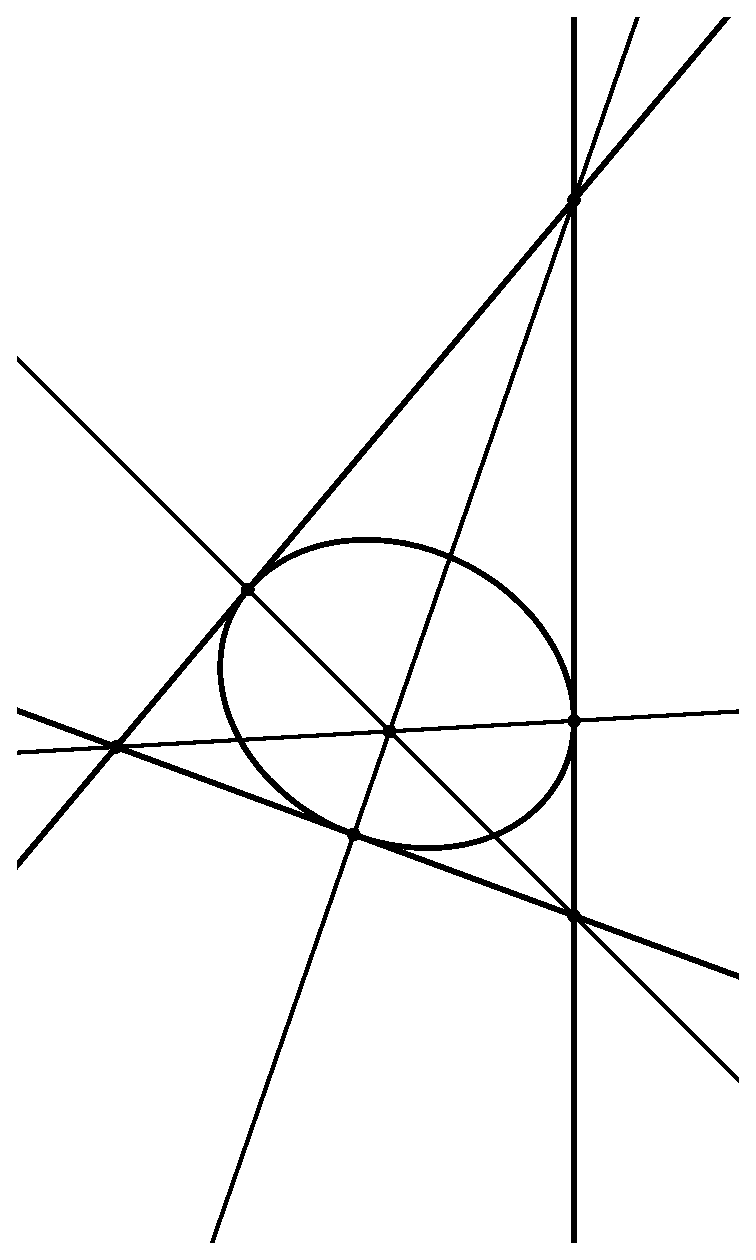
\includegraphics[scale=0.3,angle=270]{cevaconic.eps}
\caption{Exercise \ref{cevaconic}(a)}
\end{figure}

\begin{exer}\label{cevaconic}\hspace{2em}
\begin{itemize}
\item[(a)] Let $ABC$ be a triangle, let $D$ be a point on $BC$, let $E$ be a point on $CA$, and let $F$ be a point of $AB$. Show that the lines $AD,BE,CF$ meet in a point if and only if there is a conic $\omega$ which is tangent to $BC$ at $D$, tangent to $CA$ at $E$, and tangent to $AB$ at $F$.
\item[(b)] Let $ABC$ be a triangle and let $P$ be a point not lying on any edge of $ABC$. Let $U,X$ be points on $BC$ with $X = r_{(A)(P)(B\;C)}(U)$, let $V,Y$ be points on $CA$ with $Y = r_{(B)(P)(A\;C)}(V)$, and let $W,Z$ be points on $AB$ with $Z = r_{(C)(P)(A\;B)}(W)$. Show that $U,V,W,X,Y,Z$ lie on a conic.
\end{itemize}
\end{exer}

\begin{exer}[Holden Mui] Suppose $\Omega, \omega_1, \omega_2$ are conics such that $\Omega$ is tangent to $\omega_1$ at $A$ and $B$ and $\Omega$ is tangent to $\omega_2$ at $C$ and $D$. Let $P = AB\cap CD$, and let $X,Y,Z,W$ be the four points of intersection between $\omega_1$ and $\omega_2$.
\begin{itemize}
\item[(a)] Show that there is a way to order $X,Y,Z,W$ such that $XZ \cap YW = P$.

\item[(b)] Show that if $X,Y,Z,W$ are ordered as in (a), then the four lines $AB, CD; XZ, YW$ are harmonic.
\end{itemize}
\end{exer}

\begin{figure}[!htb]
\centering
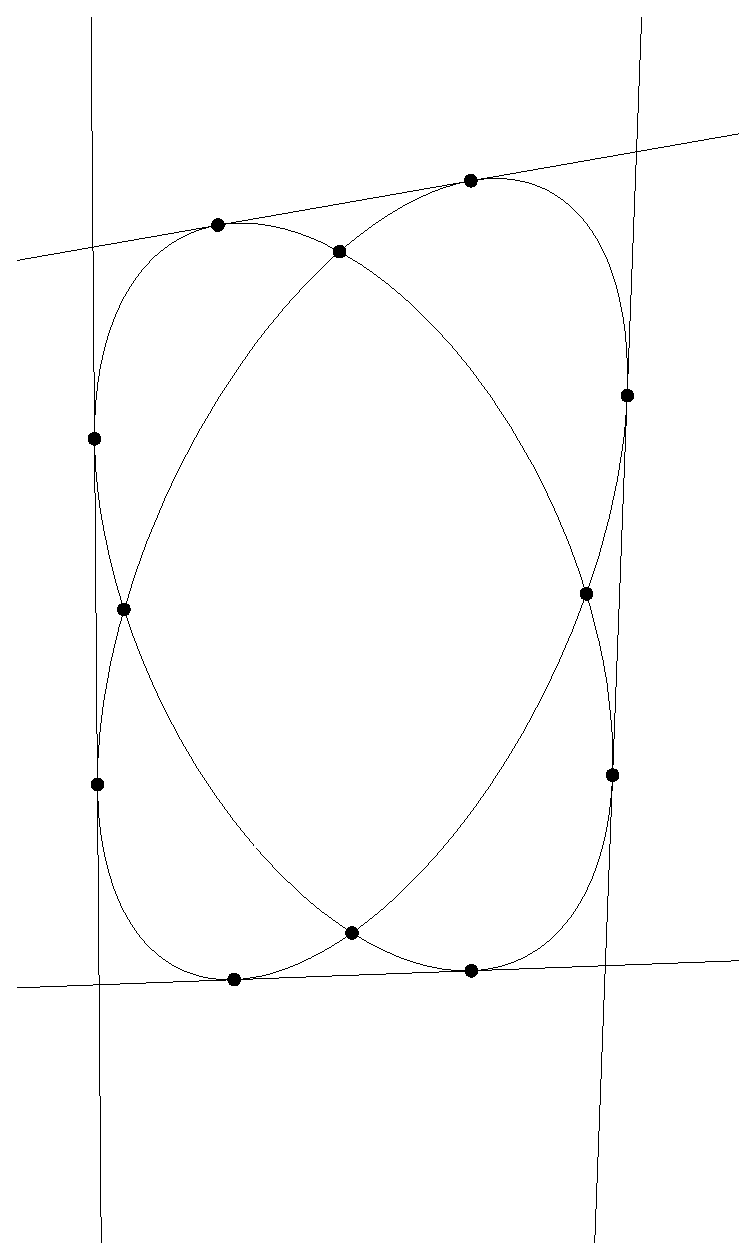
\includegraphics[scale=0.4,angle=270]{conictangents.eps}
\caption{Exercise \ref{conictangents}}
\end{figure}

\begin{exer}\label{conictangents}\hspace{2em}
\begin{itemize}
\item[(a)] Given points $A,B,C,D$ and a line $e$, there are two conics $\omega,\Omega$ passing through $A,B,C,D$ and tangent to $e$. Construct the other three common tangent lines $f,g,h$ to the conics $\omega,\Omega$ using only the points $A,B,C,D$, the line $e$, and a straightedge.

\item[(b)] Show that if you order $e,f,g,h$ correctly, you have
\[
(A,B;C,D)_\omega = (e,f;g,h)_\Omega.
\]

\item[(c)] Show that polar maps send projectively orthogonal pairs of conics to projective orthogonal pairs of conics.
\end{itemize}
\end{exer}

\begin{figure}[!htb]
\centering
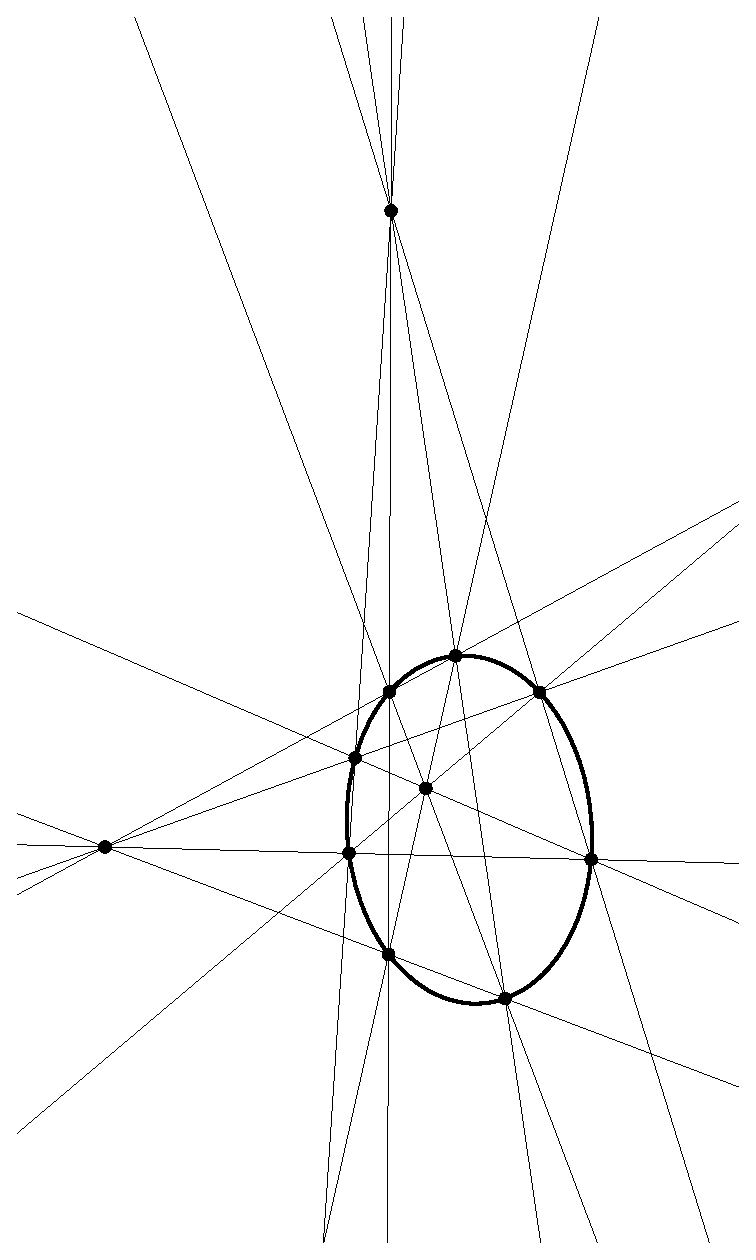
\includegraphics[scale=0.5,angle=270]{fourpairs.eps}
\caption{Exercise \ref{fourpairs}}
\end{figure}

\begin{exer}\label{fourpairs} Suppose that $A,B,C,D,E,F,G,H$ are eight distinct points in the plane such that the four lines $AB, CD, EF, GH$ meet in a point, the four lines $AC, BD, EG, FH$ meet in a point, and the four lines $AD, BC, EH, FG$ meet in a point. Show that $A,B,C,D,E,F,G,H$ all lie on a single conic.
\end{exer}

\begin{figure}[!htb]
\centering
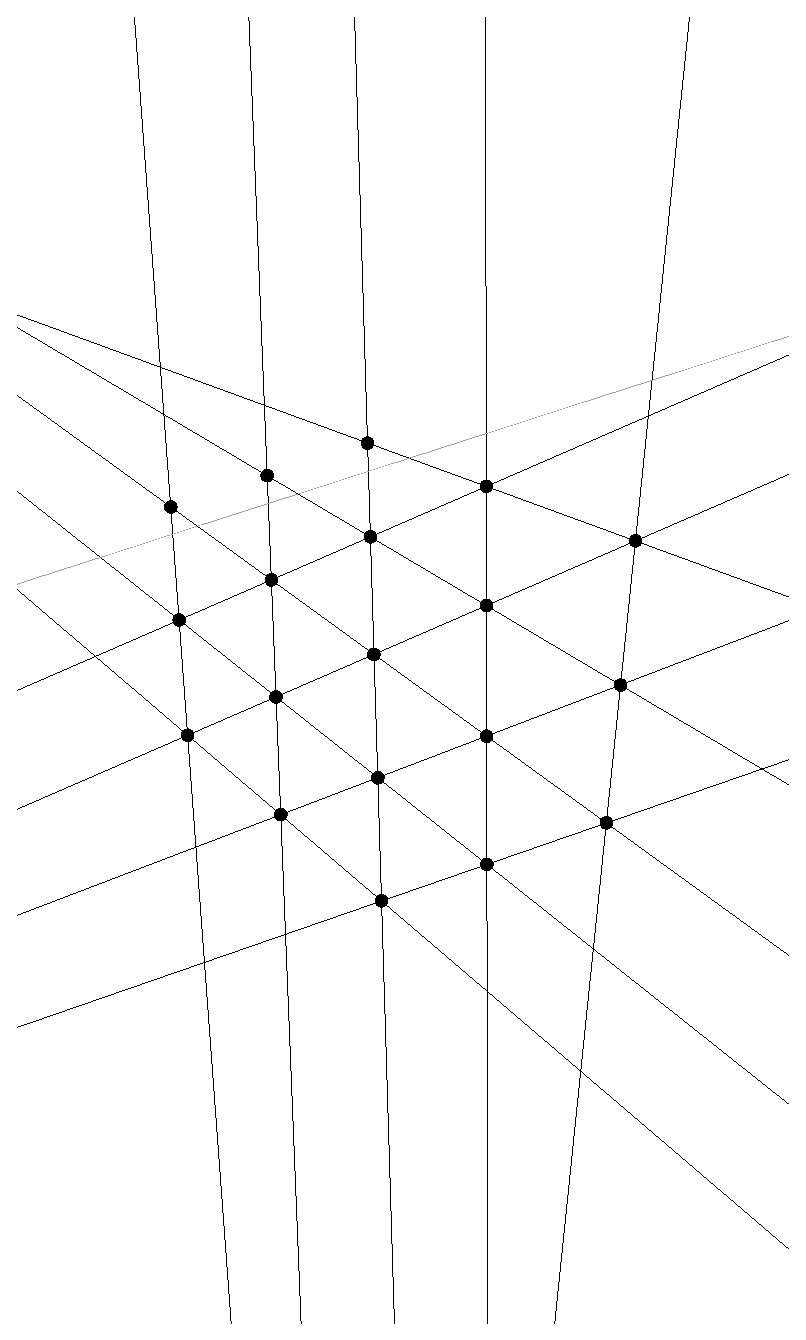
\includegraphics[scale=0.5,angle=270]{triangulargrid.eps}
\caption{Triangular grid lemma}
\end{figure}

\begin{exer}[Triangular grid lemma] Let $a_1,a_2,a_3,a_4,b_1,b_2$ be six distinct lines. Let $c_1$ be the line through $a_3\cap b_1$ and $a_2\cap b_2$. Let $c_2$ be the line through $a_4\cap b_1$ and $a_3\cap b_2$. Let $b_3$ be the line through $a_1\cap c_1$ and $a_2\cap c_2$. Let $c_3$ be the line through $a_4\cap b_2$ and $a_3\cap b_3$. Let $b_4$ be the line through $a_1\cap c_2$ and $a_2\cap c_3$. Let $c_4$ be the line through $a_4\cap b_3$ and $a_3\cap b_4$. Let $b_5$ be the line through $a_1\cap c_3$ and $a_2\cap c_4$. Let $c_5$ be the line through $a_4\cap b_4$ and $a_3\cap b_5$. Show that the three points $b_1\cap c_3, b_2\cap c_4, b_3\cap c_5$ are on a line. (Hint: use Theorem \ref{cr-equal}.)
\end{exer}


\bigskip

\section{Cross ratios in other geometries}

\subsection{Cremona involutions and blow ups}

Why would someone want to blow up a perfectly good projective plane? The issue is that sometimes we have geometric correspondences which work \emph{almost} everywhere, but have a few annoying exceptions. As an example, for any pair of points $A,B$ there is an almost perfect one-to-one correspondence between points $P$ and pairs of lines $l = AP, m = BP$ through $A,B$ (respectively), given by $P = l \cap m$, with just two aggravating problems:
\begin{itemize}
\item if $P$ is on the line $AB$, then $l = AP = AB = BP = m$, and we can't recover the point $P$ from the pair of lines $l=AB, m=BA$, and
\item if $P = A$, then there are infinitely many lines which contain $A$ and $P$, so for any line $l$ through $A$, the pair $l, m=BA$ describes $P$.
\end{itemize}

Simplifying a bit, the issue is that the map from points $P$ to lines $l = AP$ through $A$ isn't always well-defined. Often, we won't be considering just a single point $P$ in isolation, but rather we will be considering a curve $\mathcal{C}$ which happens to pass through the point $A$. In this case, there is a sensible way to extend the map from points $P \in \mathcal{C}$ to lines $l = AP$ through $A$ to the case $P = A$: we just take the line $l$ to be the tangent to the curve $\mathcal{C}$ at $A$. So what we would like to do is to remember ``which direction we approached the point $A$ from'' when $P$ hits $A$, replacing the single point $A$ with the collection of all lines through $A$. This operation is called \emph{blowing up} the point $A$.

Formally, what we will do will look a little bit stupid. Instead of just having our space consist of points $P$ in the plane $\PP^2$, we will instead consider the following collection of ordered pairs:
\[
\Bl_{A}\PP^2 = \{(P, l) \mid P \in \PP^2, \{A,P\} \subset l\}.
\]
For $P \ne A$, the only line $l$ such that the ordered pair $(P,l)$ is in $\Bl_A\PP^2$ is the line $AP$, so there is a one-to-one correspondence between points in $\PP^2$ other than $A$ and points $(P,l)$ of the blown-up plane $\Bl_A\PP^2$ with $P \ne A$. On the other hand, when $P = A$, $l$ can be any line through $A$, so there is a one-dimensional family of pairs $(A,l) \in \Bl_A\PP^2$ corresponding to the point $A \in \PP^2$ - this one-dimensional family is called the \emph{exceptional line} above $A$, and written as $e_A$.

To convince ourselves that $\Bl_A\PP^2$ is an honest geometric space (and not just a formal trick), we can write it down in coordinates. Supposing that $A = [0:0:1]$, we have
\[
\Bl_A\PP^2 = \{([p:q:r], (a:b:0)) \mid ap + bq = 0\},
\]
where the third coordinate of $l = (a:b:0)$ is forced to be $0$ since $A \in l$, and the equation $ap + bq = 0$ is equivalent to $P \in l$. Concentrating on the pairs $(P,l)$ with $r, b \ne 0$, and writing $x = p/r, y = q/r$, and $s = a/b$, we see that most of $\Bl_A\PP^2$ corresponds to the surface
\[
\{(x,y,s) \mid sx + y = 0\},
\]
and the exceptional line $e_A$ corresponds to the line $s \mapsto (0,0,s)$ which is contained within this surface. This surface can be visualized as a sort of spiral staircase, where for each fixed value of $s$ we have a line $x \mapsto (x,-sx,s)$ passing through the exceptional line $e_A$. So we can visually confirm that $\Bl_A\PP^2$ ends up being a smooth two-dimensional surface, with a map $\Bl_A \PP^2 \rightarrow \PP^2$ (given by $(P,l) \mapsto P$) which is one-to-one aside from the exceptional line $e_A$, which gets crushed down to the point $A$.

The same trick can be used to blow up a sequence of points - introducing an exceptional line for every point which gets blown up - and hopefully once we blow up the right collection of points we can cure whatever defects we had in our geometric constructions which \emph{almost} worked. The main example of such a geometric construction is the Cremona involution, which generalizes the following geometric operations:
\begin{itemize}
\item isogonal (or isotomic) conjugation of a point with respect to a triangle, which fails at the vertices of the triangle, and
\item inversion around a point $O$ in the projective plane, which fails at the points $O, \fish, \bar\fish$.
\end{itemize}
The fix will require us to blow up the three points where the operation fails.

Let $A,B,C,D$ be four points in the projective plane, no three on a line. Choose projective coordinates such that $A = [1:0:0], B = [0:1:0], C = [0:0:1], D = [1:1:1]$ (one way to do this is to start with barycentric coordinates on the triangle $A,B,C$, and then rescale the coordinates to make $D = [1:1:1]$). For future reference, let $E = [-1:1:1], F = [1:-1:1], G = [1:1:-1]$ in this coordinate system.

\begin{exer} Show that $E,F,G$ satisfy $DE \cap FG = A, DF \cap EG = B, DG \cap EF = C$, and that they are uniquely determined by these conditions. Show that $E$ is the harmonic conjugate of $D$ with respect to $A, AD\cap BC$.
\end{exer}

One of the simplest nonlinear functions we can write down is the Cremona involution: if $p,q,r$ are all nonzero, it takes the point $P = [p:q:r]$ in the above coordinate system to the point
\[
f_{ABCD}(P) = \Big[\frac{1}{p}:\frac{1}{q}:\frac{1}{r}\Big].
\]
We would like to extend this to an involution of the plane. Clearing denominators, we get
\[
f_{ABCD}(P) = [qr:pr:pq],
\]
and this lets us define $f_{ABCD}(P)$ as long as no two of $p,q,r$ are $0$, i.e. as long as $P$ is not equal to one of $A,B,C$. If $P$ is on line $BC$, then $p=0$, so $f_{ABCD}(P) = [qr:0:0] = A$, and $f_{ABCD}$ is not injective. We can fix these problems by blowing up the points $A,B,C$.

\begin{defn} If $A,B,C$ are three distinct points in the projective plane, we set
\[
\Bl_{ABC}\PP^2 = \{(P,l_A,l_B,l_C)\mid P \in \PP^2, \{A,P\} \subset l_A, \{B,P\} \subset l_B, \{C,P\} \subset l_C\}.
\]
If $(P,l_A,l_B,l_C) \in \Bl_{ABC}\PP^2$ has $P \ne A,B,C$, then $l_A = AP, l_B = BP, l_C = CP$, and we write $P$ as shorthand for $(P,l_A,l_B,l_C)$. Let $e_A$ be the set of points $(P,l_A,l_B,l_C)$ in $\Bl_{ABC}\PP^2$ with $P = A$, that is,
\[
e_A = \{(A,l,AB,AC) \mid A\in l\},
\]
and define $e_B, e_C$ similarly. If $(A,l,AB,AC)\in e_A$, we write $(A,l)$ as shorthand for it. If $P = (A,l)$, we write $AP$ as shorthand for $l$. The three lines $e_A, e_B, e_C$ are called the \emph{exceptional lines} above $A,B,C$. We say that a curve $\omega$ passing through $A$ intersects the exceptional line $e_A$ in the point $(A,l_A)$ if line $l_A$ is tangent to $\omega$ at $A$.
\end{defn}

In coordinates, we have
\[
\Bl_{ABC}\PP^2 = \{([p:q:r],(0:a:b),(c:0:d),(e:f:0))\mid aq+br = cp+dr = ep+fq = 0\}.
\]

\begin{prop} The map $[p:q:r]\mapsto [\frac{1}{p}:\frac{1}{q}:\frac{1}{r}]$, defined for $p,q,r \ne 0$, extends to an involution $f_{ABCD} : \Bl_{ABC}\PP^2 \rightarrow \Bl_{ABC}\PP^2$. The extended involution $f_{ABCD}$ takes $e_A$ (resp. $e_B, e_C$) bijectively to $BC$ (resp. $AC, AB$). The fixed points of $f_{ABCD}$ are $D,E,F,G$, and we have $f_{ABCD} = f_{ABCE} = f_{ABCF} = f_{ABCG}$.
\end{prop}
\begin{proof} In coordinates, if $P = ([p:q:r],(0:a:b),(c:0:d),(e:f:0))$ we set
\[
f_{ABCD}(P) = \begin{cases}([aq:ap:-bp],(0:b:a),(d:0:c),(f:e:0)) & \mbox{if }p\ne 0,\\([-cq:dr:dq],(0:b:a),(d:0:c),(f:e:0)) & \mbox{if }q\ne 0,\\ ([er:-fr:ep],(0:b:a),(d:0:c),(f:e:0)) & \mbox{if }r\ne 0.\end{cases}
\]
Checking that this is well-defined, along with checking the other claims of the proposition, is left as an easy exercise to the reader.
\end{proof}

\begin{rem} More generally, for any three homogeneous polynomials $f(p,q,r),g(p,q,r),h(p,q,r)$ of the same degree having no common factor we can define a map
\[
[p:q:r] \rightarrow [f(p,q,r):g(p,q,r):h(p,q,r)],
\]
which is well-defined whenever $f,g,h$ are not simultaneously zero. Such a map is called a \emph{rational map}. It is called \emph{birational} if it is usually one-to-one - in this case you can write down a rational function which inverts it whenever both are defined. Noether and Castelnuovo have proved that every birational map $\PP^2\rightarrow \PP^2$ can be built out of projective transformations and Cremona involutions.
\end{rem}

\begin{prop} Let $A,B,C,D,E,F,G$ be such that $A = DE\cap FG, B = DF\cap EG, C = DG\cap EF$, and suppose that $f_{ABCD}(P) = Q$. Then we have
\[
(AP,AQ;DE,FG) = (BP,BQ;DF,EG) = (CP,CQ;DG,EF) = -1.
\]
In other words, $AQ$ is the harmonic conjugate of $AP$ with respect to $AD, AF$, and similarly for $BQ, CQ$.
\end{prop}
\begin{proof} By symmetry, it's enough to show that $(AP,AQ;DE,FG) = -1$. In the coordinate system described above, suppose that $AP = (0:a:b)$. We then have $DE = (0:1:-1), FG = (0:1:1), AQ = (0:b:a)$, so
\[
(AP,AQ;DE,FG) = (a/b,b/a;-1,1) = -1.\qedhere
\]
\end{proof}

\begin{ex} Let $G$ be the centroid of triangle $ABC$, and suppose $f_{ABCG}(P) = Q$. Let $FED$ have parallel sides to $ABC$, such that $A$ is the midpoint of $DE$, $B$ is the midpoint of $DF$, and $C$ is the midpoint of $EF$. Let $M = AG\cap BC, X = AP \cap BC, Y = AQ \cap BC,\infty = AD\cap BC$. Then
\[
(X,Y;\infty,M) = (AP,AQ;DE,FG) = -1,
\]
so $X$ is the reflection of $Y$ across $M$, the midpoint of $BC$. Similarly, $BP\cap AC$ is the reflection of $BQ\cap AC$ across the midpoint of $AC$, etc. The point $Q$ is called the \emph{isotomic conjugate} of $P$.
\end{ex}

\begin{cor}\label{cremona-cross} Let $f = f_{ABCD}$. For any four points $P,Q,R,S\in \Bl_{ABC}\PP^2$ we have
\[
(AP,AQ;AR,AS) = (Af(P),Af(Q);Af(R),Af(S)).
\]
\end{cor}
\begin{proof} Harmonic conjugation preserves the cross ratio.
\end{proof}

\begin{thm}\label{cremona-conic} Let $l$ be a line which does not pass through any of $A,B,C$. Then $f_{ABCD}(l)$ is a \emph{circumconic}, that is, a conic passing through all three of $A,B,C$. Conversely, if $\omega$ is a circumconic then $f_{ABCD}(\omega)$ is a line which does not pass through any of $A,B,C$.
\end{thm}
\begin{proof} Write $f = f_{ABCD}$, and let $P,Q,R$ be any three points on $l$. Let $S = l\cap BC$, so that $f(S) \in e_A$. By the Corollary, we have
\[
(Bf(P),Bf(Q);Bf(R),BA) = (P,Q;R,S) = (Cf(P),Cf(Q);Cf(R),CA),
\]
so $f(R)$ lies on the conic $\omega$ through $A,B,C,f(P),f(Q)$. The converse is left as an exercise.
\end{proof}

\begin{exer} Let $I$ be the incenter of triangle $ABC$. The map $f_{ABCI}$ is called \emph{isogonal conjugation}.
\begin{itemize}
\item[(a)] Show that $f_{ABCI}(\fish) = \bar\fish$.

\item[(b)] Let $\Omega$ be the circumcircle of triangle $ABC$. Show that $f_{ABCI}(\Omega)$ is the line at infinity.

\item[(c)] Let $m$ be the median through $A$. Show that $f_{ABCI}(m)$ passes through the pole of $BC$ with respect to $\Omega$. (Hint: show that the intersections of $m, BC, AB, AC$ with the line at infinity are harmonic, then apply $f_{ABCI}$.)

\item[(d)] Let $\omega$ be the circumcircle of triangle $BCI$. Show that $f_{ABCI}(\omega) = \omega$.
\end{itemize}
\end{exer}

\begin{exer}  Write $f = f_{ABCD}$, let $l$ be a line which doesn't pass through any of $A,B,C$, let $\omega = f(l)$, and let $P,Q,R,S$ be any four points on $l$. Show that
\[
(P,Q;R,S) = (f(P),f(Q);f(R),f(S))_\omega.
\]
\end{exer}

\begin{exer} Let $A,B,C,D$ be in general position, and let $\omega$ be a conic passing through $A$, $B$, and $C$. Let $X$ be the second intersection of the line $AD$ with the conic $\omega$, and let $U$ be the intersection between the line $BC$ and the tangent to $\omega$ at $X$. Show that $U \in f_{ABCD}(\omega)$. In particular, if we define points $V \in AC, W \in AB$ similarly, then $U,V,W$ are collinear.
\end{exer}

\begin{thm}\label{cremona-two} If $\omega$ is a conic which passes through $B$ and $C$ but not $A$, then $f_{ABCD}(\omega)$ is also a conic passing through $B$ and $C$ but not $A$. We have $f_{ABCD}(\omega) = \omega$ if and only if $\omega$ either passes through $D$ and $E$ or passes through $F$ and $G$.
\end{thm}
\begin{proof} Write $f = f_{ABCD}$, and let $P,Q,R,S$ be any four points on $\omega$. By Corollary \ref{cremona-cross}, we have
\[
(Bf(P),Bf(Q);Bf(R),Bf(S)) \stackrel{B}{=} (P,Q;R,S)_\omega \stackrel{C}{=} (Cf(P),Cf(Q);Cf(R),Cf(S)),
\]
so $B,C,f(P),f(Q),f(R),f(S)$ are on a conic. If $f(\omega)$ passed through $A$, then $\omega$ would need to be tangent to $BC$ at either $B$ or $C$, which is impossible.

Note that if $f(\omega) = \omega$ then $f$ defines an involution from $\omega$ to itself, and so $f$ must fix exactly two points of $\omega$, which can't both be contained in the same line through $B$ or $C$. Conversely, suppose for instance that $D,E$ are on $\omega$, and let $X$ be any other point on $\omega$. The conic through $B,C,D,X,f(X)$ is sent to itself, so it must contain $E$. Thus $f(X)$ must be on $\omega$.
\end{proof}

\subsubsection{Aside: some basic intersection theory}

We recall (without proof) a famous theorem of B\'ezout.

\begin{thm}[B\'ezout] If $\Omega,\omega$ are distinct curves in $\PP^2$ defined by irreducible polynomial equations of degrees $m,n$, respectively, then the number of intersection points between $\Omega$ and $\omega$ is exactly $mn$, if you count points ``with multiplicity'' and remember to include imaginary points and points at infinity.
\end{thm}

In particular, any two curves in $\PP^2$ meet in at least one point. $\Bl_{ABC}\PP^2$ doesn't have this property: for instance, the line $AB$ doesn't intersect either of the lines $e_C, BC$ in $\Bl_{ABC}\PP^2$. Luckily, it's easy to modify B\'ezout's theorem to make it work for $\Bl_{ABC}\PP^2$.

\begin{defn} If $\omega$ is a curve in $\Bl_{ABC}\PP^2$ defined by an irreducible polynomial equation of degree $m$, which passes through $A,B,C$ with multiplicities $a,b,c$, respectively, we say that $\omega$ is a \emph{curve of type} $(m,-a,-b,-c)$. If $\omega = e_A$, we say that $\omega$ is a curve of type $(0,1,0,0)$, and similarly $e_B$ has type $(0,0,1,0)$, $e_C$ has type $(0,0,0,1)$.
\end{defn}

\begin{thm}\label{intersection} If $\Omega,\omega$ are distinct irreducible algebraic curves in $\Bl_{ABC}\PP^2$ of types $(m,p,q,r), (n,x,y,z)$, then the number of intersection points between $\Omega$ and $\omega$ in $\Bl_{ABC}\PP^2$ is exactly $mn - px - qy - rz$, if you count points ``with multiplicity'' and remember to include imaginary points and points at infinity.
\end{thm}

\begin{defn} If $\omega$ has type $(m,p,q,r)$, then the \emph{self-intersection number} of $\omega$ is defined to be $m^2 - p^2 - q^2 - r^2$.
\end{defn}

\begin{prop}\label{cremona-type} If $\omega$ has type $(m,p,q,r)$ then $f_{ABCD}(\omega)$ has type $(2m+p+q+r,-m-q-r,-m-p-r,-m-p-q)$.
\end{prop}

\begin{exer}
\begin{itemize}
\item[(a)] Prove Proposition \ref{cremona-type}.

\item[(b)] Using Proposition \ref{cremona-type} and Theorem \ref{intersection}, check that the number of intersection points between $\omega$ and $\Omega$ is the same as the number of intersection points between $f_{ABCD}(\omega)$ and $f_{ABCD}(\Omega)$. In particular, the self-intersection number of $\omega$ is the same as the self-intersection number of $f_{ABCD}(\omega)$.

\item[(c)] Use Proposition \ref{cremona-type} to give another proof of Theorem \ref{cremona-conic}.

\item[(d)] Find all curves in $\Bl_{ABC}\PP^2$ which have self-intersection number at most $0$.
\end{itemize}
\end{exer}


%\subsubsection{Inversion and spherical geometry}


\subsection{Hyperbolic geometry}

There are many models of hyperbolic geometry. The easiest ones to understand are the models which live inside disks in the inversive plane $\CC\PP^1$.

\begin{defn} A \emph{disk} in $\CC\PP^1$ is a circle or line $\Omega \subseteq \CC\PP^1$, together with a choice of one of the two connected components of $\CC\PP^1 \setminus \Omega$, which we call the \emph{interior} of the disk (the other connected component of $\CC\PP^1$ is called the \emph{exterior} of the disk). The circle $\Omega$ is the \emph{boundary} of the disk.
\end{defn}

Note that the choice of which region of $\CC\PP^1\setminus\Omega$ should be the interior and which should be the exterior is arbitrary, since an inversion around the center of $\Omega$ (or a reflection across $\Omega$, if $\Omega$ is a line) interchanges these two regions. So we really need to explicitly specify which region should be considered the interior of the disk in order to be unambiguous. When $\Omega$ is a circle, generally people take the interior of $\Omega$ to be the region of $\CC\PP^1$ which does not contain the point at infinity - this way, the disk can be drawn using a finite amount of paper.

\begin{defn} Let $D$ be a disk in $\CC\PP^1$ with boundary $\Omega$. The associated \emph{disk model} of hyperbolic geometry works as follows:
\begin{itemize}
\item the \emph{points} of the disk model consist of the points in the interior of $D$,
\item for every circle $\omega$ which intersects $\Omega$ at a $90$-degree angle, the set $\omega \cap D$ is a \emph{hyperbolic line} of the disk model, and
\item every point on the boundary $\Omega$ is a \emph{point at infinity} (aka a \emph{rimpoint}) of the disk model.
\end{itemize}
The \emph{angle} between hyperbolic lines $\omega_1\cap D, \omega_2\cap D$ are computed in the disk model by computing the ordinary angle between $\omega_1$ and $\omega_2$ at their point of intersection inside $D$; distances are more complicated and will be defined later. The \emph{symmetries} of the disk model are defined to be the set of M\"obius transformations and complex conjugates of M\"obius transformations of $\CC\PP^1$ which send $D$ bijectively to itself (note that these are all angle-preserving, so our definition of angles is compatible with our definition of symmetries).
\end{defn}

In order to be a legitimate geometry, our model should satisfy some basic properties.

\begin{prop}\label{hyperbolic-lines} Suppose $D$ is a disk in $\CC\PP^1$, and let $P \ne Q$ be points in $D$. Then there is a unique hyperbolic line $\ell = \omega \cap D$ which goes through $P$ and $Q$.
\end{prop}
\begin{proof} We can assume without loss of generality that the boundary $\Omega$ of $D$ is a straight line, by inverting around a point on $\Omega$ if necessary. Let $p$ be the perpendicular bisector of $PQ$: if $p$ intersects $\Omega$ at a finite point $O$ then $\omega$ must be the circle with center $O$ and radius $OP$. If $p$ is parallel to $\Omega$, then $\omega$ must be the line $PQ$.
\end{proof}

\begin{prop} If $D$ is a disk in $\CC\PP^1$ and $\ell, m$ are hyperbolic lines of $D$, then $\ell$ and $m$ intersect in at most one point of $D$.

If $\ell$ meets the boundary of $D$ at $X$ and $Y$, and $m$ meets the boundary of $D$ at $U$ and $V$, then $\ell$ and $m$ intersect in the interior of $D$ if and only if $(X,Y;U,V) < 0$.
\end{prop}
\begin{proof} Suppose that $P \in \ell \cap m$, and that $\ell = \alpha \cap D$ and $m = \beta \cap D$, where $\alpha, \beta$ are circles or lines in $\CC\PP^1$. Then inversion around the center of the disk $D$ (or reflecting across its boundary, if the boundary is a line) sends $\alpha$ and $\beta$ to themselves by Proposition \ref{hyperbolic-lines}, so it sends $P$ to the second intersection point between $\alpha$ and $\beta$. As a consequence, the second intersection point of $\alpha$ and $\beta$ is either on the exterior of $D$, or is $P$ itself (if $P$ is on the boundary of $D$).

There are two very different ways to prove the second statement. The straightforward way is to apply a M\"obius transformation which takes $X$ to $0$, $Y$ to $\infty$, and $U$ to $1$, at which point the statement becomes obvious. The more visual way is to note that $(X,Y;U,V) < 0$ exactly when $X$ and $Y$ \emph{separate} the points $U$ and $V$ along the boundary of the disk $D$. Therefore, if $(X,Y;U,V) < 0$, then the number of intersection points (counted with multiplicity) between \emph{any} smooth path connecting $X$ to $Y$ within $D$ and any smooth path connecting $U$ to $V$ within $D$ must be odd, for purely topological reasons, while if $(X,Y;U,V) > 0$ then the number of intersection points within $D$ must be even. Since the number of intersection points within $D$ is at most one, this proves the second claim.
\end{proof}

\begin{prop} Suppose $D$ is a disk in $\CC\PP^1$, $P,Q$ are points in the interior of $D$, and $\ell, m$ are hyperbolic lines with $P \in \ell$ and $Q \in m$. Then there are exactly four symmetries of the disk model which take $P$ to $Q$ and $\ell$ to $m$.
\end{prop}
\begin{proof} Let $\Omega$ be the boundary of $D$, let $A$ and $B$ be the intersections of $\ell$ with $\Omega$, and let $C$ and $D$ be the intersections of $m$ with $\Omega$. Then there is a unique M\"obius transformation $f$ which takes $A$ to $C$, $B$ to $D$, and $P$ to $Q$. Thus we have $f(\ell) = m$ and $f(P) = Q$, and we need to check that $f(\Omega) = \Omega$. By the Proposition \ref{hyperbolic-lines}, $\Omega$ is the unique circle or line which is perpendicular to $\ell$ at $A$ and $B$. Therefore $f(\Omega)$ is the unique circle or line which is perpendicular to $m$ at $C$ and $D$, which is also $\Omega$. The other symmetries which take $P$ to $Q$ and $\ell$ to $m$ are the M\"obius transformation which takes $A$ to $D$, $B$ to $C$, and $P$ to $Q$, and the variants of these which involve complex conjugation.
\end{proof}

A consequence of the last proposition is that there are no symmetries of the hyperbolic plane which fix a point and a line through it, but rescale \emph{distances} by a positive amount. So unlike Euclidean geometry and projective geometry, in hyperbolic geometry all symmetries will end up being distance-preserving, once we get around to defining what hyperbolic distance \emph{is}.

The main advantages of the disk model of hyperbolic geometry are that angles are not distorted, and that the symmetries are easy to describe. A disadvantage is that if a painter was living in a three-dimensional hyperbolic space (defined as the interior of a three-dimensional ball in a similar way to the disk model), and if they were to paint what they saw as they looked at a geometric configuration in some two-dimensional hyperbolic plane (which would be a portion of a sphere which is perpendicular to the ball they lived within), then the hyperbolic lines in the picture they would paint would be perfectly straight, not curved. Of course, when a painter paints a picture of a plane, angles will generally \emph{not} be preserved in their painting. So the true \emph{projective} model of hyperbolic space will consist of the interior of a conic section, where the hyperbolic lines are perfectly straight - this is called the \emph{Klein model} of hyperbolic space, and we will go over it later.

We will start investigating the geometry of hyperbolic space by looking at the least elegant model: the upper halfplane model. The reason for starting with this model is that the calculations involving distances and areas are easiest to describe in the upper halfplane.


\subsubsection{Upper halfplane model}

The upper halfplane is a disk in $\CC\PP^1$, with boundary equal to the real line and interior corresponding to the points with positive imaginary parts. The hyperbolic lines of the upper halfplane model are just the upright semicircles which have their centers on the real line, together with the upright half-lines which are perpendicular to the real line. Points $P$ of the upper halfplane model are often written in the form $x + iy$, where $x \in \RR$ and $y > 0$.

What are the symmetries of the upper half-plane? Any M\"obius transformation that takes the real line to itself must have the form $f : z \mapsto \frac{az + b}{cz + d}$, where $a,b,c,d$ are all real numbers, with $ad \ne bc$. To see whether such a M\"obius transformation takes the upper halfplane to itself, we just need to check whether it takes the point $i$ to a point with positive imaginary part:
\[
f(i) = \frac{ai+b}{ci+d} = \frac{(ai+b)(-ci+d)}{c^2+d^2} = \frac{ac+bd + (ad - bc)i}{c^2 + d^2}.
\]
Since $c^2 + d^2 > 0$, we see that $f(i)$ has positive imaginary part if and only if $ad - bc > 0$. Since multiplying all of $a,b,c,d$ by the same thing doesn't change the M\"obius transformation but does scale the value of $ad - bc$ by a square, people usually normalize the symmetries of the upper halfplane by assuming that $ad - bc = 1$ (this is still slightly redundant: if we negate all of $a,b,c,d$, we get the same M\"obius transformation, and $ad - bc$ is still $1$). This gives us a three-dimensional family of symmetries - just enough for the symmetries to be able to take any point and line through it to any other point and line through it.

Let's dig a little deeper into the symmetries of the upper halfplane. Suppose that $f : z \mapsto \frac{az + b}{cz + d}$ with $a,b,c,d \in \RR$ and $ad - bc = 1$. What are the fixed points of $f$? Solving the equation
\[
z = \frac{az+b}{cz+d},
\]
we get
\[
cz^2 + (d-a)z - b = 0,
\]
so
\[
z = \frac{a-d \pm \sqrt{(a-d)^2 + 4bc}}{2c} = \frac{a-d \pm \sqrt{(a+d)^2 - 4}}{2c}.
\]
We get three different cases, depending on whether or not $|a+d|$ is greater than $2$, less than $2$, or equal to $2$.

If $|a+d| > 2$, then the fixed points of $f$ are both \emph{real}, that is, they are \emph{points at infinity} in the upper halfplane model. The hyperbolic line connecting these fixed points is then preserved by $f$. To understand this case better, we may as well assume that the fixed points of $f$ are at $0$ and $\infty$ (by applying a different M\"obius transformation, if necessary). In this case we must have $b = c = 0$, and $d = 1/a$, so our M\"obius transformation is just the map
\[
z \mapsto a^2z.
\]
The fact that this map is supposed to preserve hyperbolic distances gives us a hint that along the hyperbolic line from $0$ to $\infty$ (i.e., the positive part of the imaginary axis), distances will be related to the \emph{logarithm} of the imaginary part.

If $|a+d| = 2$, then the M\"obius transformation $f$ has exactly one real fixed point, at $\frac{a-d}{2c}$. Again, we may as well assume that this fixed point is at $\infty$, in which case we must have $c = 0$ and $a = d = \pm 1$. If we take $a = d = +1$ (by negating $b$ if necessary), then our M\"obius transformation $f$ is just the map
\[
z \mapsto z + b.
\]

Finally, if $|a+d| < 2$, then the M\"obius transformation $f$ has a pair of complex fixed points, which are conjugates of each other. Exactly one of these fixed points will be in the upper halfplane. We may as well assume that this fixed point is $i$, in which case the formula for $f(i)$ we had earlier implies that $c^2 + d^2 = 1$ and $ac + bd = 0$. A little algebra shows that we must have $a = d$ and $b = -c$, so we can write
\[
\begin{bmatrix}a & b\\ c & d\end{bmatrix} = \begin{bmatrix}\cos(\theta) & \sin(\theta)\\ -\sin(\theta) & \cos(\theta)\end{bmatrix}
\]
for some angle $\theta$. This can be thought of as the hyperbolic geometry analogue of a counterclockwise rotation around $i$ - but it will be a rotation of angle $2\theta$, not $\theta$, since flipping the signs of all of the entries $a,b,c,d$ does not change the M\"obius transformation. Note that if we take $\theta = \pi/2$, so that $2\theta = \pi$, then we see that the analogue of a $180$ degree rotation around $i$ is the M\"obius transformation
\[
z \mapsto -1/z.
\]
Since rotations around $i$ should certainly preserve the distance to $i$, this gives us another hint that hyperbolic distances along the positive part of the imaginary axis will be related to logarithms. In fact, we can now justify the claim that the scaling map $z \mapsto az$ should preserve hyperbolic distances: we can build this map by composing the $180$ degree rotation $z \mapsto -1/z$ around $i$ with the $180$ degree rotation $z \mapsto -a/z$ around $ai$.

Now let's think seriously about how distances should be defined in hyperbolic geometry. Let's start by thinking about infinitesimal distances: we start from a point $x + iy$, and change $x$ by $dx$ and $y$ by $dy$. Let $ds$ be the corresponding infinitesimal amount of hyperbolic distance that we travel. In ordinary Euclidean geometry, we would have $ds^2 = dx^2 + dy^2$ by the Pythagorean theorem. In a general ``smooth'' geometry, we might instead have
\[
ds^2 = \alpha(x,y)\ dx^2 + 2\beta(x,y)\ dx\ dy + \gamma(x,y)\ dy^2,
\]
where $\alpha, \beta, \gamma$ could be any (smooth) functions we like of $x$ and $y$, subject to the conditions $\alpha > 0, \gamma > 0$, and $\alpha\gamma > \beta^2$ (to guarantee that the right hand side is always positive). Since $z \mapsto z+b$ is a symmetry of our geometry, we immediately see that the functions $\alpha, \beta, \gamma$ can't depend on $x$, and are only functions of $y$:
\[
ds^2 = \alpha(y)\ dx^2 + 2\beta(y)\ dx\ dy + \gamma(y)\ dy^2.
\]
Since the map $z\mapsto az$ is a symmetry of our geometry which should preserve distances, we see that in fact $\alpha(y), \beta(y), \gamma(y)$ should all be proportional to $1/y^2$, so we can write
\[
ds^2 = \frac{\alpha\ dx^2 + 2\beta\ dx\ dy + \gamma\ dy^2}{y^2}
\]
for some constants $\alpha, \beta, \gamma$. To compute $\alpha, \beta, \gamma$, we may as well assume that $x + iy = i$, that is, $x = 0$ and $y = 1$. Since the negated complex conjugation $z \mapsto -\bar{z}$ is a symmetry of the upper halfplane, we see that when $x+iy = i$ the map $(dx,dy) \mapsto (dx,-dy)$ has to preserve distances, so $\beta = 0$. To figure out the relationship between $\alpha$ and $\gamma$, we consider the hyperbolic $90$ degree rotation around $i$, which is given by
\[
z \mapsto \frac{1+z}{1-z}.
\]
Plugging in $z = dx + i$ (and $dy = 0$) and expanding to first order in $dx$ (i.e. ignoring larger powers of $dx$), we get
\[
\frac{1 + dx + i}{1-dx - i} = \frac{(1+dx+i)(1-dx+i))}{1 + (1-dx)^2} = \frac{2i}{2-2dx} = i(1 + dx),
\]
so this $90$ degree rotation turns an infinitesimal step in the real direction into an infinitesimal step in the imaginary direction of the same length. This shows that we must have $\alpha = \gamma$, and we may as well take $\alpha = 1$, in which case our formula for infinitesimal distances becomes
\[
ds = \frac{\sqrt{dx^2 + dy^2}}{y}.
\]
Let's check that this formula really is compatible with our symmetries.

\begin{prop} Suppose that $x+iy$ is in the upper halfplane, and let $f : z \mapsto \frac{az + b}{cz + d}$ be a M\"obius transformation with $a,b,c,d \in \RR$ and $ad - bc = 1$. If
\[
f(x+ dx +i(y + dy)) = u + du + i(v + dv)
\]
to first order, then we have
\[
\frac{\sqrt{dx^2 + dy^2}}{y} = \frac{\sqrt{du^2 + dv^2}}{v}.
\]
\end{prop}
\begin{proof} First we find $u$ and $v$:
\[
\frac{a(x+iy) + b}{c(x+iy) + d} = \frac{(ax+b)(cx+d) + acy^2 + i(ad - bc)y}{(cx+d)^2 + c^2y^2} = \frac{(ax+b)(cx+d) + acy^2}{(cx+d)^2+c^2y^2} + \frac{iy}{(cx+d)^2+c^2y^2}.
\]
In particular, we have
\[
v = \frac{y}{(cx+d)^2 + c^2y^2}.
\]
Now let $z = x+iy$, so to first order we have
\[
\frac{az+b+a\ dz}{cz+d + c\ dz} = \frac{az+b}{cz+d} + \frac{a(cz+d) - (az+b)c}{(cz+d)^2}\ dz = u + iv + \frac{dz}{(cz+d)^2}.
\]
Expanding out the last term, we get
\[
du + i\ dv = \frac{dx + i\ dy}{(cx+d + icy)^2},
\]
so
\[
|du + i\ dv| = \frac{|dx + i\ dy|}{(cx+d)^2 + c^2y^2}.
\]
Thus we have
\[
\frac{\sqrt{du^2 + dv^2}}{v} = \frac{\sqrt{dx^2+dy^2}}{(cx+d)^2 + c^2y^2}\Big/\frac{y}{(cx+d)^2 + c^2y^2} = \frac{\sqrt{dx^2 + dy^2}}{y}.\qedhere
\]
\end{proof}

Intuitively, the formula for infinitesimal distances can be thought of as saying the following:
\begin{center}
As you get closer to the real line, you become smaller, in proportion to the imaginary part of your current position.
\end{center}
In particular, if we were to try to walk directly towards the real line, we would find ourselves shrinking as we did so, and as a result we would never be able to actually reach the real line. This is why we can think of the real line as the collection of ``points at infinity'' of the hyperbolic plane. Additionally, the shortest path between two points with the same imaginary parts could contain a detour through points with larger imaginary part: when we walk away from the real line, we get larger, so we can travel more quickly.

Now that we've figured out what infinitesimal distances should look like, we can figure out what the shortest path between more distant points looks like. We start by considering the easiest case: distances along the positive part of the imaginary axis.

\begin{prop} If infinitesimal distances are given by $ds = \frac{\sqrt{dx^2 + dy^2}}{y}$, then the shortest path from $ai$ to $bi$ travels directly along the positive imaginary axis and has length $|\log(b/a)|$.
\end{prop}
\begin{proof} Moving the real part back and forth on a path from $ai$ to $bi$ obviously can only increase the total distance traveled, so it's always best to travel directly along the positive imaginary axis. If $b > a$, then the length of this path is given by
\[
\int_a^b \frac{dy}{y} = \log(b) - \log(a).\qedhere
\]
\end{proof}

Using the fact that infinitesimal distances are preserved by symmetries, we can now understand the general case of shortest paths in hyperbolic space.

\begin{thm} If infinitesimal distances are given by $ds = \frac{\sqrt{dx^2 + dy^2}}{y}$, then the shortest path from $P$ to $Q$ travels directly along the hyperbolic line $\ell$ connecting $P$ to $Q$. If $\ell$ meets the real line at $X$ and $Y$, then the length of this path is equal to
\[
\Big|\log\Big((P,Q;X,Y)\Big)\Big|.
\]
\end{thm}
\begin{proof} Let $f$ be a M\"obius transformation which takes the upper halfplane to itself, maps $P$ to $i$, and maps $\ell$ to the positive imaginary axis. Since $Q \in \ell$, $Q$ is mapped to $ai$ for some real number $a$. Since $f$ preserves infinitesimal distances, $f$ turns a shortest path from $P$ to $Q$ into a shortest path from $i$ to $ai$, and the length of these shortest paths are equal. Since the shortest path from $i$ to $ai$ travels directly along $f(\ell)$, the shortest path from $P$ to $Q$ must travel directly along $\ell$. Since $f$ preserves cross ratios, the length of this path is given by
\[
|\log(a)| = \Big|\log\Big((i,ai;0,\infty)\Big)\Big| = \Big|\log\Big((f(P),f(Q);f(X),f(Y))\Big)\Big| = \Big|\log\Big((P,Q;X,Y)\Big)\Big|.\qedhere
\]
\end{proof}

Now we can make the result of the previous theorem into a definition.

\begin{defn} If $D$ is a disk in $\CC\PP^1$, points $P,Q$ are in the interior of $D$, and the hyperbolic line $\ell$ through $P$ and $Q$ meets the boundary of $D$ at points $X$ and $Y$, then the \emph{hyperbolic distance} from $P$ to $Q$ is defined to be
\[
\delta_D(P,Q) = \Big|\log\Big((P,Q;X,Y)\Big)\Big|.
\]
\end{defn}

\begin{cor} If $D$ is a disk in $\CC\PP^1$ and points $P,Q,R$ are in the interior of $D$, then the hyperbolic distances between $P,Q,$ and $R$ satisfy the triangle inequality:
\[
\delta_D(P,R) \le \delta_D(P,Q) + \delta_D(Q,R).
\]
\end{cor}

\begin{exer} Prove the triangle inequality for hyperbolic distance directly from its definition.
\end{exer}

We can also relate \emph{angles} in hyperbolic geometry to cross ratios between points at infinity.

\begin{thm} If $\ell, m$ are intersecting hyperbolic lines in the upper halfplane model such that $\ell$ meets the real line at $X$ and $Y$ and $m$ meets the real line at $U$ and $V$, and if $\ell$ is directed from $X$ to $Y$ and $m$ is directed from $U$ to $V$, then the angle $\theta$ between $\ell$ and $m$ satisfies
%\[
%\tan^2(\theta/2) = -(X,Y;U,V)
%\]
%and
\[
\cos(\theta) = \frac{1+(X,Y;U,V)}{1-(X,Y;U,V)}.
\]
In particular, the hyperbolic lines $\ell$ and $m$ meet at a right angle if and only if $X,Y,U,V$ are harmonic.
\end{thm}
\begin{proof} We may assume without loss of generality that $X$ and $Y$ are $0$ and $\infty$, i.e. that $\ell$ is the positive part of the imaginary axis. Let $u,v$ be the real numbers corresponding to the points $U$ and $V$, and note that $\ell$ and $m$ intersect if and only if $u$ and $v$ have opposite signs. Computing the power of the point $0$ with respect to the circle with diameter $UV$ in two different ways, we see that $\ell$ and $m$ intersect in the point $i\sqrt{-uv}$. Some angle chasing reveals that the angle $\theta$ between $\ell$ and the tangent to $m$ at $i\sqrt{-uv}$ is equal to twice the angle of the right triangle formed by $U, V$, and $i\sqrt{-uv}$ at $V$, which is also equal to the angle of the right triangle formed by $0$, $V$, and $i\sqrt{-uv}$ at $V$. Thus we have
\[
|\tan(\theta/2)| = \frac{\sqrt{-uv}}{|v|} = \sqrt{-\frac{u}{v}} = \sqrt{-(0,\infty;u,v)} = \sqrt{-(X,Y;U,V)}.
\]
To finish, we apply the formula
\[
\cos(\theta) = \frac{1 - \tan^2(\theta/2)}{1 + \tan^2(\theta/2)}.\qedhere
\]
\end{proof}

%\subsubsection{Poincar\'e disk model}

%\subsubsection{Klein model}


%Minkowski geometry: replace the circle of radius i at infinity with the circle of radius 1 at infinity. So in the plane, two lines are orthogonal iff their angle bisectors have slopes 1 and -1, see also: https://physics.stackexchange.com/questions/12435/einsteins-postulates-leftrightarrow-minkowski-space-for-a-layman/13621#13621


%\subsection{Finite projective planes}

%\subsubsection{Projective plane modulo $p$}

%\subsubsection{Desarguesian planes}


%\subsection{Stable degeneration}

%\bigskip

%\section{Applications of cross ratios}

%\subsection{invariants of elliptic curves}

%\subsection{dilogarithms and volumes of ideal tetrahedra}

%\subsection{percolation, conformal invariance}

%\subsection{Schwarzian derivative}

%three conic theorem!!!

\nocite{geo}
%TODO: cite Hilbert's "Foundations of Geometry"
%\bibliography{cross}
%\bibliographystyle{plain}

%\end{document}

